\documentclass[]{book}
\usepackage{lmodern}
\usepackage{amssymb,amsmath}
\usepackage{ifxetex,ifluatex}
\usepackage{fixltx2e} % provides \textsubscript
\ifnum 0\ifxetex 1\fi\ifluatex 1\fi=0 % if pdftex
  \usepackage[T1]{fontenc}
  \usepackage[utf8]{inputenc}
\else % if luatex or xelatex
  \ifxetex
    \usepackage{mathspec}
  \else
    \usepackage{fontspec}
  \fi
  \defaultfontfeatures{Ligatures=TeX,Scale=MatchLowercase}
\fi
% use upquote if available, for straight quotes in verbatim environments
\IfFileExists{upquote.sty}{\usepackage{upquote}}{}
% use microtype if available
\IfFileExists{microtype.sty}{%
\usepackage[]{microtype}
\UseMicrotypeSet[protrusion]{basicmath} % disable protrusion for tt fonts
}{}
\PassOptionsToPackage{hyphens}{url} % url is loaded by hyperref
\usepackage[unicode=true]{hyperref}
\hypersetup{
            pdftitle={Bayesian},
            pdfauthor={Bill Last Updated:},
            pdfborder={0 0 0},
            breaklinks=true}
\urlstyle{same}  % don't use monospace font for urls
\usepackage{natbib}
\bibliographystyle{apalike}
\usepackage{color}
\usepackage{fancyvrb}
\newcommand{\VerbBar}{|}
\newcommand{\VERB}{\Verb[commandchars=\\\{\}]}
\DefineVerbatimEnvironment{Highlighting}{Verbatim}{commandchars=\\\{\}}
% Add ',fontsize=\small' for more characters per line
\usepackage{framed}
\definecolor{shadecolor}{RGB}{248,248,248}
\newenvironment{Shaded}{\begin{snugshade}}{\end{snugshade}}
\newcommand{\KeywordTok}[1]{\textcolor[rgb]{0.13,0.29,0.53}{\textbf{#1}}}
\newcommand{\DataTypeTok}[1]{\textcolor[rgb]{0.13,0.29,0.53}{#1}}
\newcommand{\DecValTok}[1]{\textcolor[rgb]{0.00,0.00,0.81}{#1}}
\newcommand{\BaseNTok}[1]{\textcolor[rgb]{0.00,0.00,0.81}{#1}}
\newcommand{\FloatTok}[1]{\textcolor[rgb]{0.00,0.00,0.81}{#1}}
\newcommand{\ConstantTok}[1]{\textcolor[rgb]{0.00,0.00,0.00}{#1}}
\newcommand{\CharTok}[1]{\textcolor[rgb]{0.31,0.60,0.02}{#1}}
\newcommand{\SpecialCharTok}[1]{\textcolor[rgb]{0.00,0.00,0.00}{#1}}
\newcommand{\StringTok}[1]{\textcolor[rgb]{0.31,0.60,0.02}{#1}}
\newcommand{\VerbatimStringTok}[1]{\textcolor[rgb]{0.31,0.60,0.02}{#1}}
\newcommand{\SpecialStringTok}[1]{\textcolor[rgb]{0.31,0.60,0.02}{#1}}
\newcommand{\ImportTok}[1]{#1}
\newcommand{\CommentTok}[1]{\textcolor[rgb]{0.56,0.35,0.01}{\textit{#1}}}
\newcommand{\DocumentationTok}[1]{\textcolor[rgb]{0.56,0.35,0.01}{\textbf{\textit{#1}}}}
\newcommand{\AnnotationTok}[1]{\textcolor[rgb]{0.56,0.35,0.01}{\textbf{\textit{#1}}}}
\newcommand{\CommentVarTok}[1]{\textcolor[rgb]{0.56,0.35,0.01}{\textbf{\textit{#1}}}}
\newcommand{\OtherTok}[1]{\textcolor[rgb]{0.56,0.35,0.01}{#1}}
\newcommand{\FunctionTok}[1]{\textcolor[rgb]{0.00,0.00,0.00}{#1}}
\newcommand{\VariableTok}[1]{\textcolor[rgb]{0.00,0.00,0.00}{#1}}
\newcommand{\ControlFlowTok}[1]{\textcolor[rgb]{0.13,0.29,0.53}{\textbf{#1}}}
\newcommand{\OperatorTok}[1]{\textcolor[rgb]{0.81,0.36,0.00}{\textbf{#1}}}
\newcommand{\BuiltInTok}[1]{#1}
\newcommand{\ExtensionTok}[1]{#1}
\newcommand{\PreprocessorTok}[1]{\textcolor[rgb]{0.56,0.35,0.01}{\textit{#1}}}
\newcommand{\AttributeTok}[1]{\textcolor[rgb]{0.77,0.63,0.00}{#1}}
\newcommand{\RegionMarkerTok}[1]{#1}
\newcommand{\InformationTok}[1]{\textcolor[rgb]{0.56,0.35,0.01}{\textbf{\textit{#1}}}}
\newcommand{\WarningTok}[1]{\textcolor[rgb]{0.56,0.35,0.01}{\textbf{\textit{#1}}}}
\newcommand{\AlertTok}[1]{\textcolor[rgb]{0.94,0.16,0.16}{#1}}
\newcommand{\ErrorTok}[1]{\textcolor[rgb]{0.64,0.00,0.00}{\textbf{#1}}}
\newcommand{\NormalTok}[1]{#1}
\usepackage{longtable,booktabs}
% Fix footnotes in tables (requires footnote package)
\IfFileExists{footnote.sty}{\usepackage{footnote}\makesavenoteenv{long table}}{}
\usepackage{graphicx,grffile}
\makeatletter
\def\maxwidth{\ifdim\Gin@nat@width>\linewidth\linewidth\else\Gin@nat@width\fi}
\def\maxheight{\ifdim\Gin@nat@height>\textheight\textheight\else\Gin@nat@height\fi}
\makeatother
% Scale images if necessary, so that they will not overflow the page
% margins by default, and it is still possible to overwrite the defaults
% using explicit options in \includegraphics[width, height, ...]{}
\setkeys{Gin}{width=\maxwidth,height=\maxheight,keepaspectratio}
\IfFileExists{parskip.sty}{%
\usepackage{parskip}
}{% else
\setlength{\parindent}{0pt}
\setlength{\parskip}{6pt plus 2pt minus 1pt}
}
\setlength{\emergencystretch}{3em}  % prevent overfull lines
\providecommand{\tightlist}{%
  \setlength{\itemsep}{0pt}\setlength{\parskip}{0pt}}
\setcounter{secnumdepth}{5}
% Redefines (sub)paragraphs to behave more like sections
\ifx\paragraph\undefined\else
\let\oldparagraph\paragraph
\renewcommand{\paragraph}[1]{\oldparagraph{#1}\mbox{}}
\fi
\ifx\subparagraph\undefined\else
\let\oldsubparagraph\subparagraph
\renewcommand{\subparagraph}[1]{\oldsubparagraph{#1}\mbox{}}
\fi

% set default figure placement to htbp
\makeatletter
\def\fps@figure{htbp}
\makeatother

\usepackage{booktabs}
\usepackage{amsthm}
\makeatletter
\def\thm@space@setup{%
  \thm@preskip=8pt plus 2pt minus 4pt
  \thm@postskip=\thm@preskip
}
\makeatother

\title{Bayesian}
\author{Bill Last Updated:}
\date{24 January, 2020}

\begin{document}
\maketitle

{
\setcounter{tocdepth}{1}
\tableofcontents
}
\chapter*{Preface: Motivation}\label{my-section}
\addcontentsline{toc}{chapter}{Preface: Motivation}

All the notes I have done here are about bayesian. While I have tried my
best, probably there are still some typos and errors. Please feel free
to let me know in case you find one. Thank you!

\chapter{Bayesian - 1}\label{bayesian---1}

The following is the part of the class note that I took from the online
course of ``Bayesian Statistics: From Concept to Data Analysis.''
(\url{https://www.coursera.org/learn/bayesian-statistics/home/welcome})

Important note: All the notes here are just for my own study purpose. I
do not clain any copyright. You can use it for study purpose as well,
but not for any business purposes.

\section{Frequentist perspective}\label{frequentist-perspective}

\[\theta = \{ fair , loaded \}\] \[x \sim Bin (5, \theta)\]
\[\begin{aligned} f(x|\theta) &=\begin{cases} \binom{5}{x} (\frac{1}{2})^5 & if \; \theta=fair  \\ \binom{5}{x} (0.7)^x(0.3)^{5-x} & if \;  \theta=loaded  \end{cases} \\ &= \binom{5}{x} (\frac{1}{2})^5 I_{\{\theta=fair \}}+\binom{5}{x} (0.7)^x(0.3)^{5-x}I_{\{\theta=loaded \}}\end{aligned}\]

When \(x=2\)

\[f(\theta | x=2)=\begin{cases} \binom{5}{x} (\frac{1}{2})^5 = 0.3125& if \; \theta=fair  \\ \binom{5}{x} (0.7)^x(0.3)^{5-x} = 0.1323& if \;  \theta=loaded  \end{cases}\]
Thus, based on MLE, it suggests that it should be ``fair'', since it has
a greater probablity if we observe 2 head out of 5 trials.

However, we can not know the following probability: given that we
observe \(x=2\), what is the probability that \(\theta\) is fair?

\[P(\theta=fair | X=2)\] From the frequentist's perspective, the coin is
the fixed coin. And thus, the probablity of \(P(\theta=fair|x=2)\) is
equal to \(P(\theta=fair)\).

\[P(\theta=fair|x=2)=P(\theta=fair)\] As,

\[P(\theta=fair) \in C(0,1) (i.e., either \; 0 \; or \; 1)\]

\section{Bayesian perspective}\label{bayesian-perspective}

Prior \(P(loaded)=0.6\)

\[\begin{aligned} f(\theta | X) &= \frac{f(x|\theta) f(\theta)}{\sum_{\theta} f(x|\theta)f(\theta)} \\ &=\frac{\binom{5}{x} [(\frac{1}{2})^5 \times 0.4 \times I_{\{\theta=fair \}}+ (0.7)^x(0.3)^{5-x} \times 0.6 \times I_{\{\theta=loaded \}}]}{\binom{5}{x} [(\frac{1}{2})^5 \times 0.4 + (0.7)^x(0.3)^{5-x} \times 0.6]}  \end{aligned}\]

\[\begin{aligned} f(\theta |X=2) &=\frac{0.0125 I_{\{\theta=fair \}}+0.0079 I_{\{\theta=loaded \}} }{0.0125+0.0079} \\ &= 0.612 I_{\{\theta=fair \}} + 0.388 I_{\{\theta=loaded \}} \end{aligned}\]

Thus, we can say that:

\[P(\theta=loaded | X=2)=0.388\] We can change the prior, and get
different posterior probabilities:

\[P(\theta=loaded)=\frac{1}{2} \rightarrow P(\theta=loaded | X=2)=0.297\]
\[P(\theta=loaded)=\frac{9}{10} \rightarrow P(\theta=loaded | X=2)=0.792\]

\section{Continous parameters}\label{continous-parameters}

In the examples above, \(\theta\) is discrete. In contrast, the examples
below use continous \(\theta\).

\[f(\theta |y)=\frac{f(y|\theta) f(\theta)}{f(y)}=\frac{f(y|\theta) f(\theta)}{\int f(y|\theta)f(\theta)d\theta}=\frac{likelihood \times prior}{normalizing-constant} \propto likelihood \times prior\]

Note that, the posterior is a PDF of \(\theta\), which is not in the
function of \(f(y)\). Thus, removing the denominator (i.e., the
normalizing constant) does not change the form of the posterior.

\subsection{Uniform}\label{uniform}

Suppose that \(\theta\) is the probablity of a coin getting head. We
could assign a uniform distribution.

\[\theta \sim U[0,1]\]

\[f(\theta)=I_{ \{0 \leqq \theta \leqslant 1 \}}\] (It is interesting to
see how to write the pdf for uniform distribution.)

\[f(\theta | Y=1)= \frac{\theta^1(1-\theta)^0 I_{\{0 \leqq \theta \leqslant 1\}}}{\int_{-\infty}^{+\infty} \theta^1(1-\theta)^0 I_{\{0 \leqq \theta \leqslant 1\}} d\theta}=\frac{\theta I_{\{0 \leqq \theta \leqslant 1 \}}}{\int_0^1 \theta d\theta}=2\theta I_{ \{0 \leqq \theta \leqslant 1\}}\]

If we ignore the normalizing constant, we will get

\[f(\theta | Y=1) \propto \theta^1(1-\theta)^0 I_{ \{0 \leqq \theta \leqslant 1\} }=\theta I_{ \{0 \leqq \theta \leqslant 1\} }\]

Thus, we can see that with vs.~without the noramlizing constant is the
``2''.

\subsection{Uniform: prior versus
posterior}\label{uniform-prior-versus-posterior}

When \(\theta\) follows uniform distribution:

\textbf{Prior}

\[P(0.025 <\theta<0.975)=0.95\] \[P( 0.05< \theta )=0.95\]
\textbf{Posterior}

\[P(0.025<\theta<0.975)=\int_{0.025}^{0.975} 2\theta d\theta=0.95\]
\[P(0.05<\theta)=1-P(\theta <0.05)=\int_{0}^{0.05} 2\theta d\theta=1-0.05^2=0.9975\]

Thus, we can see that, while \(P(0.025<\theta<0.975)\) is the same for
prior and posterior, \(P(0.05<\theta)\) is not the same.

\subsection{Uniform: equal tailed versus
HPD}\label{uniform-equal-tailed-versus-hpd}

\textbf{Equal tailed}

\[P(\theta < q|Y=1)=\int_0^q 2\theta d\theta=q^2\]
\[P(\sqrt{0.025}<\theta<\sqrt{0.975}|Y=1)=P(0.158<\theta<0.987)=0.95\]
We can say that: there's a 95\% probability that \(\theta\) is in
between 0.158 and 0.987.

\textbf{Highest Posterior Density}

\[P(\theta > \sqrt{0.05}|Y=1)=P(\theta >0.224|Y=1)=0.95\]

\section{Bernoulli/binomial likelihood with uniform
prior}\label{bernoullibinomial-likelihood-with-uniform-prior}

\[\begin{aligned}  f(\theta | Y=1) &= \frac{\theta^{\sum y_i}(1-\theta)^{\sum n-y_i} I_{\{0 \leqq \theta \leqslant 1\}}}{\int_{-\infty}^{+\infty} \theta^{\sum y_i}(1-\theta)^{n-\sum y_i} I_{\{0 \leqq \theta \leqslant 1\}} d\theta} \\ &=\frac{\theta^{\sum y_i}(1-\theta)^{\sum n-y_i} I_{\{0 \leqq \theta \leqslant 1\}}}{\frac{\Gamma(\sum y_i+1)\Gamma(n-\sum y_i+1)}{\Gamma(n+2)} \int_{-\infty}^{+\infty} \frac{\Gamma(n+2)}{\Gamma(\sum y_i+1)\Gamma(n-\sum y_i+1)} \theta^{\sum y_i}(1-\theta)^{n-\sum y_i} I_{\{0 \leqq \theta \leqslant 1\}} d\theta} \\ &= \frac{\Gamma(n+2)}{\Gamma(\sum y_i+1)\Gamma(n-\sum y_i+1)}\theta^{\sum y_i}(1-\theta)^{\sum n-y_i} I_{\{0 \leqq \theta \leqslant 1\}}  \end{aligned} \]

Thus,

\[\theta | y \sim Beta (\sum y_i+1, n-\sum y_i +1)\]

\textbf{Side note:} \(Beta(1,1)=Uniform(0,1)\):

\(Beta(\alpha,\beta)=\frac{x^{\alpha-1}(1-x)^{\beta-1}}{B(\alpha,\beta)} I_{\{0 \leqq x \leqslant 1\}}\)

Thus, we can get the following since the support for beta distribution
is \([0,1]\):

\(Beta(1,1)=\frac{x^0(1-x)^0}{B(\alpha,\beta)}=1\times I_{\{0 \leqq x \leqslant 1\}}\)

\section{Conjugate priors}\label{conjugate-priors}

As noted above, beta prior (or, Uniform) leads to beta posterior. In a
more general sense, Beta prior always leads to beta posterior.

For instance,

\[\begin{aligned} f(\theta |y) \propto f(y|\theta)f(\theta)&=\theta^{\sum y_i}(1-\theta)^{\sum n-y_i}\frac{\theta^{\alpha-1}(1-\theta)^{\beta-1}}{B(\alpha,\beta)} I_{\{0 \leqq \theta \leqslant 1\}} \\ &=\frac{1}{B(\alpha, \beta)}\theta^{\sum y_i+\alpha-1}(1-\theta)^{\sum n-y_i+\beta-1} I_{\{0 \leqq \theta \leqslant 1\}} \\ &\propto  \theta^{\sum y_i+\alpha-1}(1-\theta)^{\sum n-y_i+\beta-1} I_{\{0 \leqq \theta \leqslant 1\}} \end{aligned}\]
Thus,

\[f(\theta |y) \sim Beta(\alpha+\sum y_i,\beta+\sum n-y_i)\] Conjugate
prior: prior and posterior share the same distribution. As we can see,
both the data and the prior contribute to the posterior.

For the prior of \(Beta(\alpha, \beta)\), the mean is

\[Mean_{prior}=\frac{\alpha}{\alpha+\beta}\]

Posterior mean is,

\[\begin{aligned} Mean_{posterior}&= \frac{\alpha+\sum y_i}{\alpha+\sum y_i+\beta+n-\sum y_i} \\ &=\frac{\alpha+\sum y_i}{\alpha+\beta+n} \\ &= \frac{\alpha+\beta}{\alpha+\beta+n}\frac{\alpha}{\alpha+\beta}+\frac{n}{\alpha+\beta+n}\frac{\sum y_i}{n} \\ &= Weight_{prior} \times Mean_{prior}+Weight_{data} \times Mean_{data}\end{aligned}\]

\textbf{Side Note}

\begin{enumerate}
\def\labelenumi{(\arabic{enumi})}
\tightlist
\item
  Binomial proportion confidence interval:
\end{enumerate}

\[\hat{p} +/- 1.96 \sqrt{\frac{\hat{p}(1-\hat{p})}{n}}\] (2) Mean of
Beta distribution:

\[\frac{\alpha}{\alpha+\beta}\] (3) Plot of Beta distribution

\begin{Shaded}
\begin{Highlighting}[]
\CommentTok{# Method 1}
\NormalTok{x<-}\KeywordTok{seq}\NormalTok{(}\DecValTok{0}\NormalTok{,}\DecValTok{1}\NormalTok{,}\DataTypeTok{length=}\DecValTok{200}\NormalTok{)}
\KeywordTok{plot}\NormalTok{(x,}\KeywordTok{dbeta}\NormalTok{(x,}\DecValTok{1}\NormalTok{,}\DecValTok{5}\NormalTok{),}\DataTypeTok{type =} \StringTok{"l"}\NormalTok{)}
\end{Highlighting}
\end{Shaded}

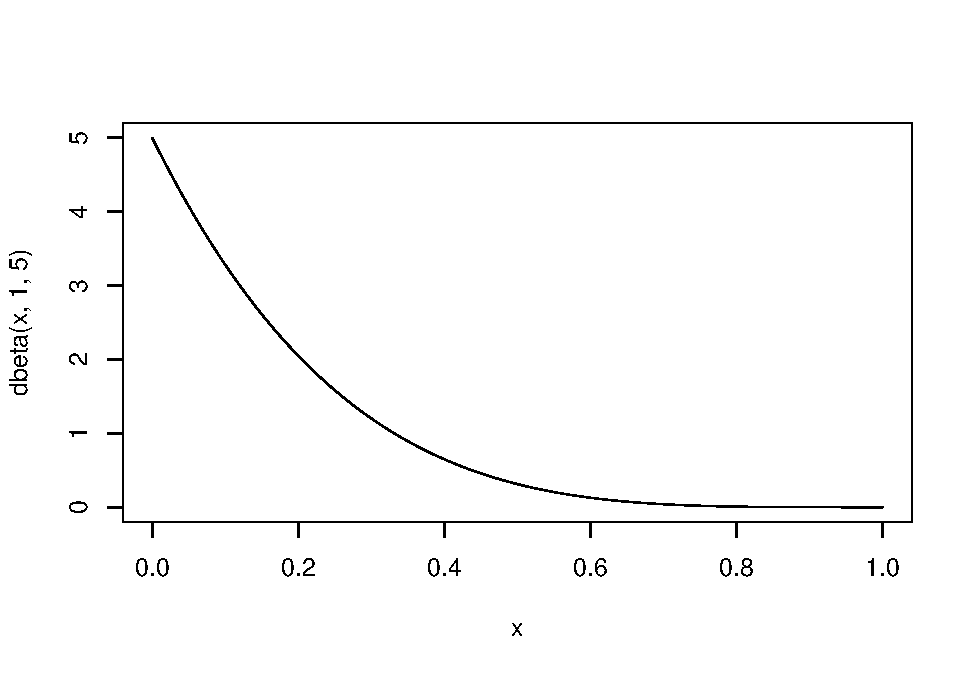
\includegraphics{bookdown-demo_files/figure-latex/unnamed-chunk-1-1.pdf}

\begin{Shaded}
\begin{Highlighting}[]
\CommentTok{# Method 2}
\NormalTok{x2<-}\KeywordTok{rbeta}\NormalTok{(}\DecValTok{200}\NormalTok{,}\DecValTok{1}\NormalTok{,}\DecValTok{5}\NormalTok{)}
\KeywordTok{hist}\NormalTok{(x2,}\DataTypeTok{prob =} \OtherTok{TRUE}\NormalTok{)}
\KeywordTok{lines}\NormalTok{(}\KeywordTok{density}\NormalTok{(x2))}
\end{Highlighting}
\end{Shaded}

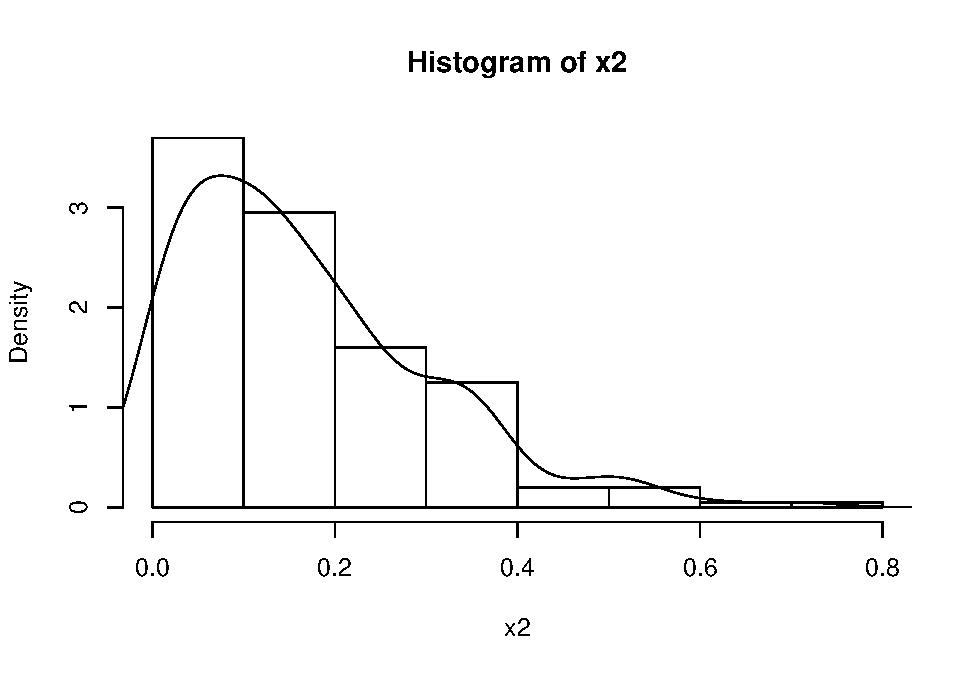
\includegraphics{bookdown-demo_files/figure-latex/unnamed-chunk-1-2.pdf}

\section{Poisson distribution}\label{poisson-distribution}

Pmf of Poisson distribution:

\[Pois (\lambda) \sim \frac{\lambda^k e^{-\lambda}}{k!}\]

We can replace \(k\) with the notation of \(y\), and assume that we
observe \(n\) \(y_i\):
\[y_i \sim \frac{\lambda^{y_i} e^{-\lambda}}{y_i!}\]

\[f(y|\lambda)=\frac{\lambda^{\sum y_i} e^{- n \lambda}}{\prod_{i=1}^n y_i !}\]

We assume that \(\lambda\) follows Gamma distribution (i.e.,Gamma
prior):

\[\lambda \sim \Gamma(\alpha, \beta)\] The pdf for Gamma distribution
is:

\[\frac{\beta^{\alpha}}{\Gamma(\alpha)}x^{\alpha-1}e^{-\beta x}\]

Thus, the posterior is as follows:

\[\begin{aligned} f(\lambda | y) &\propto f(y|\lambda)f(\lambda) \\ &=\frac{\lambda^{\sum y_i} e^{- n \lambda}}{\prod_{i=1}^n y_i !} \times \frac{\beta^{\alpha}}{\Gamma(\alpha)}\lambda^{\alpha-1}e^{-\beta \lambda} \\ &\propto \lambda^{\sum y_i}e^{- n \lambda} \times \lambda^{\alpha-1}e^{-\beta \lambda} \\ &=\lambda^{(\alpha+\sum y_i)-1}e^{- (\beta+n) \lambda} \end{aligned}\]
Thus, the posterior is:

\[\Gamma(\alpha + \sum y_i, \beta+n)\]

As we know that, the mean of prior for Gamma is
\(\frac{\alpha}{\beta}\). Thus, we can get the mean for the posterior
for Gamma is:

\[\begin{aligned} &=\frac{\alpha+\sum y_i}{\beta+n} \\ &= \frac{\beta}{\beta+n} \frac{\alpha}{\beta}+\frac{n}{\beta+n} \frac{\sum y_i}{n} \end{aligned}\]
To determine the prior of \(\alpha\) and \(\beta\):

\begin{enumerate}
\def\labelenumi{(\arabic{enumi})}
\tightlist
\item
  Prior mean \(\frac{\alpha}{\beta}\)
\end{enumerate}

\begin{enumerate}
\def\labelenumi{(\alph{enumi})}
\tightlist
\item
  Prior std. dev. \(\frac{\sqrt \alpha}{\beta}\)
\item
  Effective sample size \(\beta\)
\end{enumerate}

\begin{enumerate}
\def\labelenumi{(\arabic{enumi})}
\setcounter{enumi}{1}
\tightlist
\item
  Vague prior Small \(\varepsilon >0\):
  \(\Gamma (\varepsilon,\varepsilon)\) . Thus, the posterior mean is
  primarily driven by the data:
\end{enumerate}

\[\frac{\varepsilon + \sum y_i}{\varepsilon + n} \approx \frac{ \sum y_i}{n} \]

\begin{enumerate}
\def\labelenumi{(\arabic{enumi})}
\item
  As we know, beta prior lead the Bernoulli trial to a beta posterior.
  That is, we know \(f(\theta|y)=\frac{f(y|\theta) f(\theta)}{f(y)}\).
  What is the prior predictive distribution of \(f(y)\)?
\item
  If Beta is Beta (3,3), what is the prior predictive probablity that we
  wil observe \(y=0\) in the next trial?
\end{enumerate}

\section{Exponential data}\label{exponential-data}

For instance, suppose that on average you need to wait for 10 minutes
for a fast food delivery, and thus we can assume that
\(y \sim Exp(\lambda)\). Furthermore, we assume that the prior
\(\lambda\) follows Gamma distribution \(Gamma(\alpha, \beta)\), thus it
is with a mean of \(\frac{\alpha}{\beta}=\frac{1}{10}\).

\[if \; \; \Gamma (100, 1000)\] (Note that, it has a mean of
\(\frac{100}{1000}=\frac{1}{10}\)).

Thus, we can get:

\[\begin{aligned} f(\lambda | y) &\propto f(y|\lambda) f(\lambda) \\ &\propto \lambda e^{-\lambda y} \lambda^{\alpha-1}e^{-\beta \lambda} \\ &\propto \lambda^{(\alpha+1)-1} e^{-(\beta+y)\lambda } \end{aligned}\]
Thus, we get

\[\lambda |y \sim \Gamma (\alpha+1,\beta+y)\] Thus, if we observe a data
point that we need to wait for 12 minutes for a fast food delivery, we
can update the posterior:

\[\lambda |y \sim \Gamma (101,1012)\] Thus, the mean for the posterior
is

\[\frac{101}{1012}=\frac{1}{10.02}\]

\textbf{Note:}

\begin{enumerate}
\def\labelenumi{(\arabic{enumi})}
\item
  Typically, we know that the pdf of Gamma is
  \(\frac{\beta^{\alpha}}{\Gamma(\alpha)}x^{\alpha-1}e^{-\beta x}\). We
  replace \(x\) with \(\lambda\) since now the random variable of \(x\)
  is to represent the parameter \(\lambda\) in the exponential
  distribution.
\item
  In the above, we drop the constant part
  (\(\frac{\beta^{\alpha}}{\Gamma(\alpha)}\)) in the Gamma distribution
  as long as it does not include \(x\) (i.e., \(\lambda\)).
\item
  Suppose that you have 4 observations in total, then
\end{enumerate}

\[\begin{aligned} f(\lambda | y) &\propto f(y_1|\lambda)f(y_2|\lambda)f(y_3|\lambda)f(y_4|\lambda)    f(\lambda) \\ &\propto \lambda e^{-\lambda y_1} \lambda e^{-\lambda y_2}\lambda e^{-\lambda y_3} \lambda e^{-\lambda y_4}   \lambda^{\alpha-1}e^{-\beta \lambda} \\ &\propto \lambda^{(\alpha+4)-1} e^{-(\beta+\sum_{i=1}^4 y_i)\lambda } \end{aligned}\]
Thus, the generalized form is as follows:

\[\lambda^{(\alpha+n)-1} e^{-(\beta+\sum_{i=1}^n y_i)\lambda }\]

\section{Normal likelihood}\label{normal-likelihood}

\subsection{When variance is known}\label{when-variance-is-known}

\[x_i \sim N(\mu, \sigma_0^2)\] (\(\sigma_0\) is assumed to be known.
Thus, the only unknown parameter is \(\mu\).)

The conjugate prior for normal distribution is normal distribution
itself.

\[f(\mu |x) \sim f(x|\mu) f(\mu)\]

Assume that \[\mu \sim N(m_0,s_0^2)\]

\[\mu|x \sim N(\frac{\frac{n \bar{x}}{\sigma_o^2}+\frac{m_o}{S_0^2}}{\frac{n}{\sigma_0^2}+\frac{1}{s_0^2}},\frac{1}{\frac{n}{\sigma_0^2}+\frac{1}{s_0^2}})\]

Thus, where

\[\begin{aligned} \frac{\frac{n \bar{x}}{\sigma_o^2}+\frac{m_o}{S_0^2}}{\frac{n}{\sigma_0^2}+\frac{1}{s_0^2}}&=\frac{\frac{n \bar{x}}{\sigma_o^2}}{\frac{n}{\sigma_0^2}+\frac{1}{s_0^2}}+\frac{\frac{m_o}{S_0^2}}{\frac{n}{\sigma_0^2}+\frac{1}{s_0^2}}\\ &=\frac{n}{n+\frac{\sigma_0^2}{s_0^2}} \bar{x}+\frac{\frac{\sigma_0^2}{S_0^2}}{n+\frac{\sigma_0^2}{s_0^2}}m_o \end{aligned}\]
\textbf{Note:}

\begin{enumerate}
\def\labelenumi{(\arabic{enumi})}
\item
  As we can see, the posterior mean is a weighted mean -- a combination
  of prior mean and sample mean.
\item
  When n is larger, the sample mean \(\bar{x}\) gets more weight.
\item
  For the prior mean \(m_0\), the smaller the prior variance \(s_0^2\)
  is, the prior mean gets more weight. If the prior variance \(s_0^2\)
  is big, the prior mean will get less weight in the final posterior
  mean.
\end{enumerate}

\subsection{When variance is unknown}\label{when-variance-is-unknown}

\[x_i | \mu, \sigma^2 \sim N (\mu, \sigma^2)\]

\[\mu | \sigma^2 \sim N(m, \frac{\sigma^2}{w})\]

\textbf{Side note:}

\(w=\frac{\sigma^2}{\sigma_{\mu}^2}\) effective sample size

\[\sigma^2 \sim \Gamma^{-1}(\alpha, \beta)\]

Thus, we can get that,

\[\sigma^2 | x\sim \Gamma^{-1}(\alpha+\frac{n}{2}, \beta+\frac{1}{2} \sum_{i=1}^{n}(x_i-\bar{x})^2+\frac{nw}{2(n+w)}(\bar{x}-m)^2)\]

\[\mu| \sigma^2,x \sim N(\frac{n \bar{x}+wm}{n+w},\frac{\sigma^2}{n+w})\]

Where,

\(\frac{n \bar{x}+wm}{n+w} = \frac{w}{n+w}m+\frac{n}{n+w}\bar{x}\)

\[\mu |x \sim t - distribution \]

\section{Non-informative priors}\label{non-informative-priors}

\subsection{Bernoulli}\label{bernoulli}

\(Y_i \sim B(\theta)\)

\[\theta \sim U[0,1]= Beta (1,1)\] (Effective sample size is 1+1=2)

If we get \(Beta(\frac{1}{2},\frac{1}{2})\) and \(Beta(0.001, 0.001)\)
have less impact on the posterior.

Improper prior, for instance, THe prior \[Beta (0,0)\]
\[f(\theta) \propto \theta ^{-1}(1-\theta)^{-1}\]

In this case,

\[f(\theta| y) \propto \theta^{y-1}(1-\theta)^{n-y-1} \sim Beta(y, n-y)\]

Posterior mean: \(\frac{y}{n}=\hat{\theta}\)

\subsection{Gaussian}\label{gaussian}

\[Y_i \sim N(\mu, \sigma^2)\]

Vague prior:

\[\mu \sim N(0, 1000000^2)\] or,

\[f(\mu) \sim 1\]

\[\begin{aligned} f(\mu | y) &\propto f(y|\mu)f(\mu) \\ &\propto exp(-\frac{1}{2 \sigma^2} \sum (y_i-\mu)^2) \times 1 \\ &\propto exp(-\frac{1}{2 \frac{\sigma^2}{n}} \sum (y_i-\bar{y})^2) \end{aligned}\]

Thus,

\[\mu | y \sim N(\bar{y}, \frac{\sigma^2}{n})\]

This is exactly the same as the esitimate from MLE estimate.

\textbf{NOTE}

In case that the variance is unknown,

\[f(\sigma^2) \propto \frac{1}{\sigma^2}\]

This is equivalent to the following:

\[\Gamma ^{-1}(0,1)\] Thus the posteiro for \(\sigma^2\)

\[\sigma^2|y \sim \Gamma ^{-1} (\frac{n-1}{2},\frac{1}{2} \sum (y_i-\bar{y})^2)\]

\section{Jeffreys Priors}\label{jeffreys-priors}

Jeffreys Prior

\[f(\theta) \propto \sqrt{I(\theta)}\] For instance,

\subsection{Gaussian}\label{gaussian-1}

\[Y_i \sim (\mu, \sigma^2) \rightarrow f(\mu) \propto 1, f(\sigma^2)\propto \frac{1}{\sigma^2}\]

\subsection{Bernoulli}\label{bernoulli-1}

\[Y_i \sim B(\theta) \rightarrow f(\theta) \propto \theta ^{-\frac{1}{2}}(1-\theta)^{-\frac{1}{2}}\sim Beta(\frac{1}{2},\frac{1}{2})\]

\subsection{Side Note: Fisher
Information}\label{side-note-fisher-information}

The Fisher information (for one paramter):

\[?(\theta)=E[(\frac{d}{d\theta} log(f(X|\theta)))^2]\] The Expectation
is with respect to \(X\) with a PDF \(f(x|\theta)\).

For instance, suppose the \(X|\theta \sim N(\theta,1)\)

\[\begin{aligned} f(x|\theta) &=\frac{1}{\sqrt{2 \pi}} exp[-\frac{1}{2}(x-\theta)^2] \\ log(f(x|\theta)) &= log(\frac{1}{\sqrt{2 \pi}})-\frac{1}{2}(x-\theta)^2 \\ \frac{d}{d\theta}log(f(x|\theta)) &=x-\theta \\ (\frac{d}{d\theta}log(f(x|\theta)))^2 &=(x-\theta)^2 \\E[(\frac{d}{d\theta}log(f(x|\theta)))^2]&=(x-\theta)^2=Var(X)=1 \end{aligned}\]

\subsection{Prior predictive
distribution}\label{prior-predictive-distribution}

Prior distribution vs.~prior predictive distribution

\url{https://stats.stackexchange.com/questions/394648/differences-between-prior-distribution-and-prior-predictive-distribution}

Stochastic Processes

\url{https://www.youtube.com/watch?v=TuTmC8aOQJE}

\section{Linear regression}\label{linear-regression}

\subsection{Review}\label{review}

For single covariate of \(x\):

\[E[y]=\beta_0+\beta_1 x\] Thus,

\[Y \sim N(\beta_0+\beta_1 x, \sigma^2)\] For multiple covariates,

\[E[y]=\beta_0+\beta_1 x_1+\beta_2 x_2 + ...+ \beta_kx_k\] \textbf{Side
Note} It is interesting to think \(y\) as the expected value of of the
combination of \(\beta x\).

\subsection{\texorpdfstring{When \(\sigma^2\) is
known}{When \textbackslash{}sigma\^{}2 is known}}\label{when-sigma2-is-known}

If we use a Jeffreys prior and assume \(\sigma^2\) is known, we will get
\(\beta\) that has the same mean as the standard OLS. Assuming we only
has one covariate:

\[\beta_1|y \sim N(\frac{\sum_{i=1}^n (x_i-\bar{x})(y_i-\bar{y})}{\sum_{i=1}^n(x_i-\bar{x})^2},\frac{\sigma^2}{\sum_{i=1}^n(x_i-\bar{x})^2})\]

For mutiple covariates, we can use matrix notation,

\[\beta|y \sim N((X^tX)^{-1}X^ty,(X^tX)^{-1}\sigma^2)\]

\subsection{\texorpdfstring{When \(\sigma^2\) is
unknown}{When \textbackslash{}sigma\^{}2 is unknown}}\label{when-sigma2-is-unknown}

When both \(\beta\) and \(\sigma^2\) are unknown, the standard prior is
the non-informative Jeffreys prior:

\[f(\beta, \sigma^2) \propto \frac{1}{\sigma^2}\]

The posterior mean for \(\beta\) is the same as standard OLS estimates.
The posterior for \(\beta\) conditional on \(\sigma^2\) is the same
normal distribution when \(\sigma^2\) is known. However, the marginal
posteior distribution for \(\beta\), with \(\sigma^2\) integrated out,
is a \(t\) distribution.

The \(t\) distribution has the mean of \((X^tX)^{-1}X^ty\) and variance
matrix, \(s^2(X^tX)^{-1}\), where
\(s^2=\sum_{i=1}^n(y_i-\hat{y_i})^2/(n-k-1)\)

The variance of \(\sigma^2\) is an inverse gamma distribution

\[\sigma^2|y \sim \Gamma^{-1}(\frac{n-k-1}{2},\frac{n-k-1}{2}s^2)\]

\chapter{Bayesian - 2}\label{bayesian---2}

\section{Components of Bayesian
models}\label{components-of-bayesian-models}

\[y_i=\mu+\epsilon_i\]

Where,

\[\epsilon_i \sim N(0, \sigma^2)\]

\[y_i \sim N(\mu, \sigma^2)\] (Thus, \(y_i\) is \(=\) to a fixed \(\mu\)
plus with a \(\epsilon_i\), whereas \(y_i \sim N(\mu, \sigma^2)\). These
two expressions are not exactly the same, but they are connected.)

\textbf{Likelihood:} \(P(y|\theta)\)
(\(P(y,\theta)=P(\theta)P(y|\theta)\))

\textbf{Prior:} \(P(\theta)\)

\textbf{Posterior:}

\[P(\theta|y)=\frac{P(\theta, y)}{P(y)}=\frac{P(\theta, y)}{\int P(\theta, y)d\theta}=\frac{P(\theta)P(y|\theta)}{\int P(\theta, y)d\theta}=\frac{P(\theta)P(y|\theta)}{\int P(\theta)P(y|\theta)d\theta}\]
\textbf{Markts}

\begin{enumerate}
\def\labelenumi{(\arabic{enumi})}
\item
  The only random variables in frequentist models are the data. In
  contrast, Bayesian paradigm also uses probability to describe one's
  uncertainty about unknown model parameters.
\item
  Consider the following model for binary outcome \(y\):
\end{enumerate}

\(y_i|\theta_i \sim Bern (\theta_i), i=1,2,3...6\)

\(\theta_i |\alpha \sim Beta(a, b_0), i=1,2,3...6\)

\(\alpha \sim Exp(r_0)\)

Thus, the joint distribution of all variable:

\[\prod_{i=1}^{6}[\theta_i^{y_i}(1-\theta_i)^{1-y_i}\frac{\Gamma(a+b_0)}{\Gamma(a)\Gamma(b_0)}\theta_i^{a-1}(1-\theta_i)^{b_0-1}]r_0e^{-r_0 \alpha}\]
(Question: Why not write it as \(a_i\)?)

\section{Monte Carlo Estimation}\label{monte-carlo-estimation}

\subsection{Mean and Variance: Application of Central Limit
Theorem}\label{mean-and-variance-application-of-central-limit-theorem}

If we simulate 100 samples from a Gamma(2,1), what is the approximate
distribution of the sample average
\(\bar{x^*}=\frac{1}{100} \sum_{i=1}^{100} x_i^*\)?

As we know, based on the central limit theorem, the approximating
distribution is normal with the mean equal to the sample mean, and the
variance equal to the variance of the orignal variable divided by the
sample size. We know that the mean for Gamma(2,1) is \(\frac{2}{1}=2\)
and variance is \(\frac{2}{1^2}=2\). Thus, we know that the mean for the
distribution for \(\bar{x^*}\) is 2, whereas the variance is
\(\frac{2}{100}\). Thus, it is \(N(2,0.02)\).

Thus, we can get the generalized formula as follows:

\[\bar{\theta^*} \sim N(E(\theta), \frac{Var(\theta)}{m})\] Note that,
it is the variance for \(\bar{\theta^*}\), not \(\theta\). The
approximate for the variance for \(\theta\) is
\(\frac{1}{m}\sum(\theta_i^*-\bar{\theta^*})^2\).

The following R code is for the \(\theta\):

\begin{Shaded}
\begin{Highlighting}[]
\NormalTok{sample_data_gamma<-}\KeywordTok{rgamma}\NormalTok{(}\DecValTok{10000}\NormalTok{,}\DecValTok{4}\NormalTok{,}\DecValTok{2}\NormalTok{)}
\KeywordTok{mean}\NormalTok{(sample_data_gamma)}
\end{Highlighting}
\end{Shaded}

\begin{verbatim}
## [1] 1.985827
\end{verbatim}

\begin{Shaded}
\begin{Highlighting}[]
\KeywordTok{var}\NormalTok{(sample_data_gamma)}
\end{Highlighting}
\end{Shaded}

\begin{verbatim}
## [1] 0.9729596
\end{verbatim}

The following R code is for the \(\bar{\theta^*}\). As we can see, the
variance is 0.0016, which is close to the true value of
\(\frac{1}{1000}=0.001\).

\begin{Shaded}
\begin{Highlighting}[]
\KeywordTok{set.seed}\NormalTok{(}\DecValTok{123}\NormalTok{)}
\NormalTok{mean_c<-}\KeywordTok{c}\NormalTok{()}
\ControlFlowTok{for}\NormalTok{(i }\ControlFlowTok{in} \DecValTok{1}\OperatorTok{:}\DecValTok{10}\NormalTok{)}
\NormalTok{\{mean_c[i]<-}\KeywordTok{mean}\NormalTok{(}\KeywordTok{rgamma}\NormalTok{(}\DecValTok{1000}\NormalTok{,}\DecValTok{4}\NormalTok{,}\DecValTok{2}\NormalTok{))\}}
\KeywordTok{var}\NormalTok{(mean_c)}
\end{Highlighting}
\end{Shaded}

\begin{verbatim}
## [1] 0.001634891
\end{verbatim}

\textbf{Side Note}

Note that the definition of variance is:

\[V(x)=E[(x-\mu)^2]\]

Thus, we can calculate the variance using integral:

\[V(x)=\int (x-\mu)^2 f(x)dx\] When we using samples from the
simulation, we will get the following:

\[V(x)=\int (x-\mu)^2 f(x)dx= \frac{1}{m} \sum (x_i^*-\bar{x^*})^2\]
Thus, we can use \(Var\) function in \(R\) with simulated sample to
calculate the variance.

\subsection{Monte Carlo error (Standard
Error)}\label{monte-carlo-error-standard-error}

For the \(\bar{x^*}\), we can use the CLT to approximate how accurate
the Monte Carlo estimates are.

\[\frac{SD(sample)}{\sqrt{m}}\]

\begin{Shaded}
\begin{Highlighting}[]
\KeywordTok{set.seed}\NormalTok{(}\DecValTok{123}\NormalTok{)}
\NormalTok{sample_data_gamma<-}\KeywordTok{rgamma}\NormalTok{(}\DecValTok{10000}\NormalTok{,}\DecValTok{4}\NormalTok{,}\DecValTok{2}\NormalTok{)}

\KeywordTok{hist}\NormalTok{(sample_data_gamma, }\DataTypeTok{freq=}\OtherTok{FALSE}\NormalTok{)}
\KeywordTok{curve}\NormalTok{(}\KeywordTok{dgamma}\NormalTok{(}\DataTypeTok{x=}\NormalTok{x, }\DataTypeTok{shape=}\DecValTok{4}\NormalTok{, }\DataTypeTok{rate=}\DecValTok{2}\NormalTok{), }\DataTypeTok{col=}\StringTok{"blue"}\NormalTok{, }\DataTypeTok{add=}\OtherTok{TRUE}\NormalTok{)}
\end{Highlighting}
\end{Shaded}

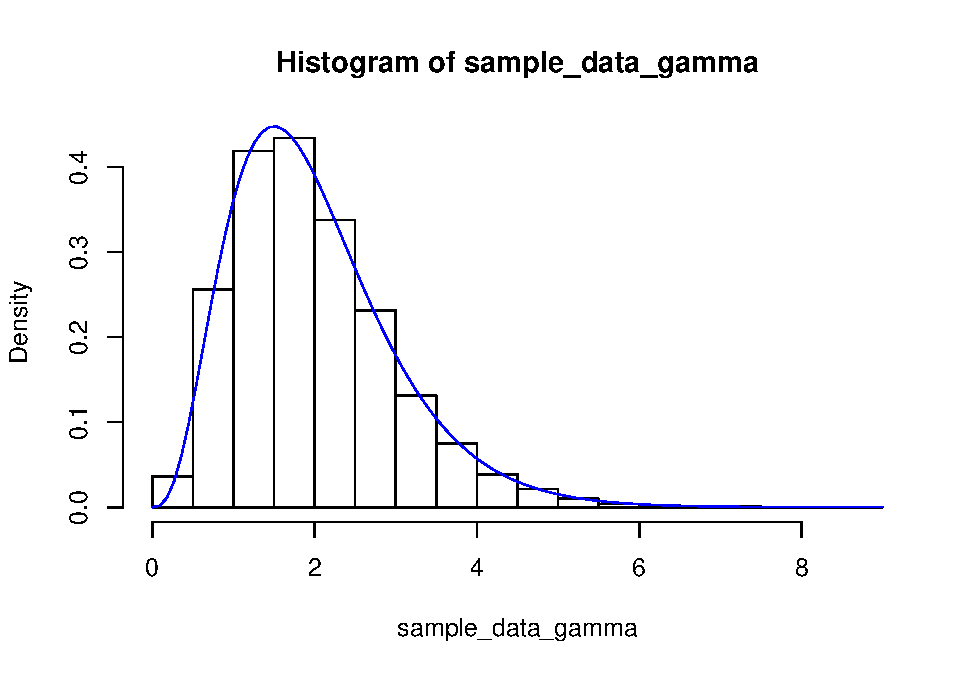
\includegraphics{bookdown-demo_files/figure-latex/unnamed-chunk-4-1.pdf}

\begin{Shaded}
\begin{Highlighting}[]
\KeywordTok{var}\NormalTok{(sample_data_gamma)}
\end{Highlighting}
\end{Shaded}

\begin{verbatim}
## [1] 0.9682145
\end{verbatim}

\begin{Shaded}
\begin{Highlighting}[]
\KeywordTok{sqrt}\NormalTok{(}\KeywordTok{var}\NormalTok{(sample_data_gamma))}
\end{Highlighting}
\end{Shaded}

\begin{verbatim}
## [1] 0.9839789
\end{verbatim}

\begin{Shaded}
\begin{Highlighting}[]
\KeywordTok{sd}\NormalTok{(sample_data_gamma) }
\end{Highlighting}
\end{Shaded}

\begin{verbatim}
## [1] 0.9839789
\end{verbatim}

\begin{Shaded}
\begin{Highlighting}[]
\KeywordTok{sd}\NormalTok{(sample_data_gamma) }\OperatorTok{/}\StringTok{ }\KeywordTok{sqrt}\NormalTok{(}\DecValTok{10000}\NormalTok{)}
\end{Highlighting}
\end{Shaded}

\begin{verbatim}
## [1] 0.009839789
\end{verbatim}

We can also calculate Standard Error for the probablity

\begin{Shaded}
\begin{Highlighting}[]
\KeywordTok{hist}\NormalTok{(sample_data_gamma)}
\end{Highlighting}
\end{Shaded}

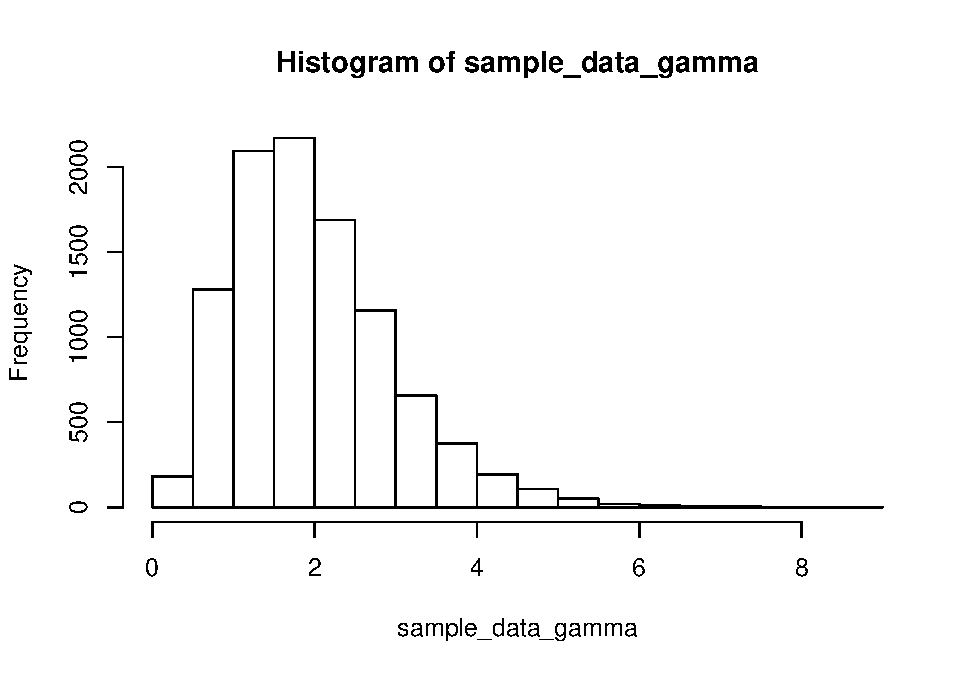
\includegraphics{bookdown-demo_files/figure-latex/unnamed-chunk-5-1.pdf}

\begin{Shaded}
\begin{Highlighting}[]
\NormalTok{se =}\StringTok{ }\KeywordTok{sd}\NormalTok{(sample_data_gamma}\OperatorTok{<}\DecValTok{5}\NormalTok{) }\OperatorTok{/}\StringTok{ }\KeywordTok{sqrt}\NormalTok{(}\DecValTok{10000}\NormalTok{)}
\NormalTok{se}
\end{Highlighting}
\end{Shaded}

\begin{verbatim}
## [1] 0.0009547917
\end{verbatim}

\subsection{Expected value and
probability}\label{expected-value-and-probability}

If you know that \(\theta \sim Beta(5,3)\), what is the approximate for
the \(E(\frac{\theta}{1-\theta})\)? You can use the following R code to
calculate it.

\begin{Shaded}
\begin{Highlighting}[]
\NormalTok{sample_data<-}\KeywordTok{rbeta}\NormalTok{(}\DecValTok{1000}\NormalTok{,}\DecValTok{5}\NormalTok{,}\DecValTok{3}\NormalTok{)}
\KeywordTok{mean}\NormalTok{(sample_data}\OperatorTok{/}\NormalTok{(}\DecValTok{1}\OperatorTok{-}\NormalTok{sample_data))}
\end{Highlighting}
\end{Shaded}

\begin{verbatim}
## [1] 2.789685
\end{verbatim}

If you want to calculate the approximate for the probability that
\(\frac{\theta}{1-\theta}\) is greater 1.

\begin{Shaded}
\begin{Highlighting}[]
\KeywordTok{mean}\NormalTok{((sample_data}\OperatorTok{/}\NormalTok{(}\DecValTok{1}\OperatorTok{-}\NormalTok{sample_data))}\OperatorTok{>}\DecValTok{1}\NormalTok{)}
\end{Highlighting}
\end{Shaded}

\begin{verbatim}
## [1] 0.789
\end{verbatim}

\subsection{Quantile}\label{quantile}

Use Monte Carlo to approximate the 0.3 quantile of N(0,1). Note that,
the idea of quantile is to quantify the probability. Thus, the number we
will get for 0.3 quantile if the value for the random variable's cdf
\(\int_{-\infty}^{quantile-number}dx\). As we can see below,
\(quantile(sample_data2,0.3)\) gets the result of -0.52, which is the
same from the \(qnorm(0.3)\). Note that, the cdf of \(pnorm(-0.52)\)
will get the probablity of \(0.3\).

\begin{Shaded}
\begin{Highlighting}[]
\NormalTok{sample_data2<-}\KeywordTok{rnorm}\NormalTok{(}\DecValTok{10000}\NormalTok{,}\DecValTok{0}\NormalTok{,}\DecValTok{1}\NormalTok{)}
\KeywordTok{quantile}\NormalTok{(sample_data2,}\FloatTok{0.3}\NormalTok{)}
\end{Highlighting}
\end{Shaded}

\begin{verbatim}
##        30% 
## -0.5260847
\end{verbatim}

\begin{Shaded}
\begin{Highlighting}[]
\KeywordTok{qnorm}\NormalTok{(}\FloatTok{0.3}\NormalTok{)}
\end{Highlighting}
\end{Shaded}

\begin{verbatim}
## [1] -0.5244005
\end{verbatim}

\begin{Shaded}
\begin{Highlighting}[]
\KeywordTok{pnorm}\NormalTok{(}\OperatorTok{-}\FloatTok{0.52}\NormalTok{)}
\end{Highlighting}
\end{Shaded}

\begin{verbatim}
## [1] 0.3015318
\end{verbatim}

\subsection{Prior predictive distributions
(Marginalization)}\label{prior-predictive-distributions-marginalization}

\[y|\theta \sim Bin(10, \theta)\] \[\theta \sim Beta(2,2)\]

Simulate:

\begin{enumerate}
\def\labelenumi{(\arabic{enumi})}
\item
  \(\theta^*\) from beta
\item
  Given \(\theta\), draw \(y_i^* \sim Bin(10, \theta_i^*)\)
\item
  Get pairs (\(y_i^*\),\(\theta_i^*\))
\end{enumerate}

\begin{Shaded}
\begin{Highlighting}[]
\NormalTok{m=}\DecValTok{1000}

\NormalTok{y=}\KeywordTok{numeric}\NormalTok{(m)}
\NormalTok{phi=}\KeywordTok{numeric}\NormalTok{(m)}

\ControlFlowTok{for}\NormalTok{ (i }\ControlFlowTok{in} \DecValTok{1}\OperatorTok{:}\NormalTok{m)}
\NormalTok{\{}
\NormalTok{  phi[i]=}\KeywordTok{rbeta}\NormalTok{(}\DecValTok{1}\NormalTok{,}\DataTypeTok{shape1=}\DecValTok{2}\NormalTok{,}\DataTypeTok{shape2 =} \DecValTok{2}\NormalTok{)}
\NormalTok{  y[i]=}\KeywordTok{rbinom}\NormalTok{(}\DecValTok{1}\NormalTok{,}\DataTypeTok{size=}\DecValTok{10}\NormalTok{,}\DataTypeTok{prob =}\NormalTok{ phi[i])}
\NormalTok{\}}

\CommentTok{# we can use vector method}

\NormalTok{phi=}\KeywordTok{rbeta}\NormalTok{(m,}\DataTypeTok{shape1 =} \DecValTok{2}\NormalTok{,}\DataTypeTok{shape2 =} \DecValTok{2}\NormalTok{)}
\NormalTok{y=}\KeywordTok{rbinom}\NormalTok{(m,}\DataTypeTok{size=}\DecValTok{10}\NormalTok{,}\DataTypeTok{prob =}\NormalTok{ phi)}
\KeywordTok{table}\NormalTok{(y)}\OperatorTok{/}\NormalTok{m}
\end{Highlighting}
\end{Shaded}

\begin{verbatim}
## y
##     0     1     2     3     4     5     6     7     8     9    10 
## 0.038 0.064 0.100 0.110 0.124 0.112 0.131 0.117 0.093 0.069 0.042
\end{verbatim}

\begin{Shaded}
\begin{Highlighting}[]
\CommentTok{# The marginal distribution of y}
\KeywordTok{plot}\NormalTok{(}\KeywordTok{table}\NormalTok{(y)}\OperatorTok{/}\NormalTok{m)}
\end{Highlighting}
\end{Shaded}

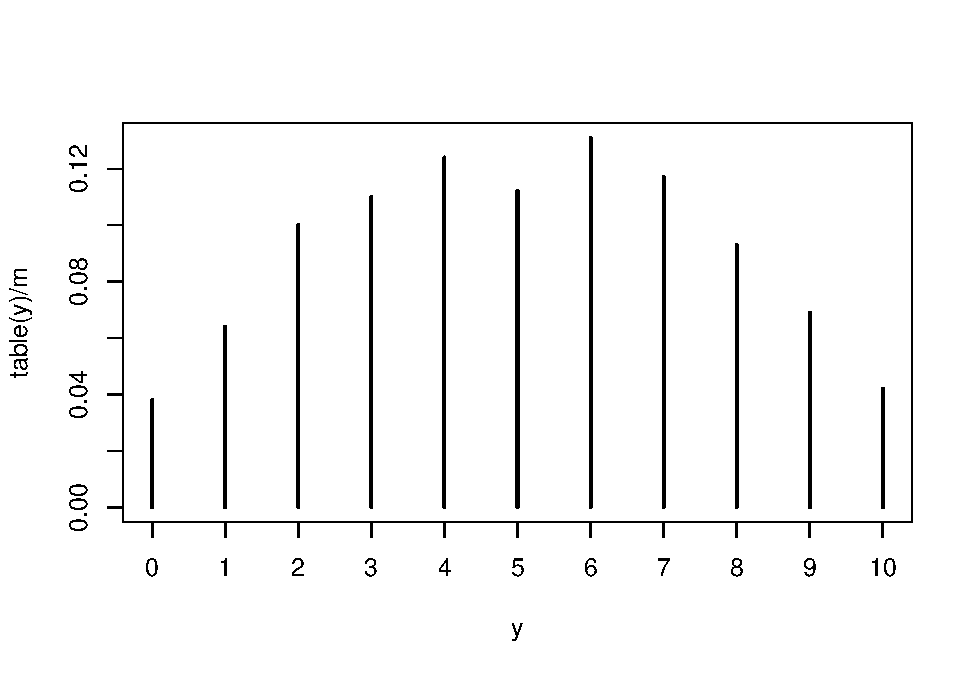
\includegraphics{bookdown-demo_files/figure-latex/unnamed-chunk-9-1.pdf}

\begin{Shaded}
\begin{Highlighting}[]
\CommentTok{# Another way to plot }
\KeywordTok{plot}\NormalTok{(}\KeywordTok{prop.table}\NormalTok{(}\KeywordTok{table}\NormalTok{(y)), }\DataTypeTok{ylab=}\StringTok{"P(y)"}\NormalTok{, }\DataTypeTok{main=}\StringTok{"Marginal distribution of y"}\NormalTok{)}
\end{Highlighting}
\end{Shaded}

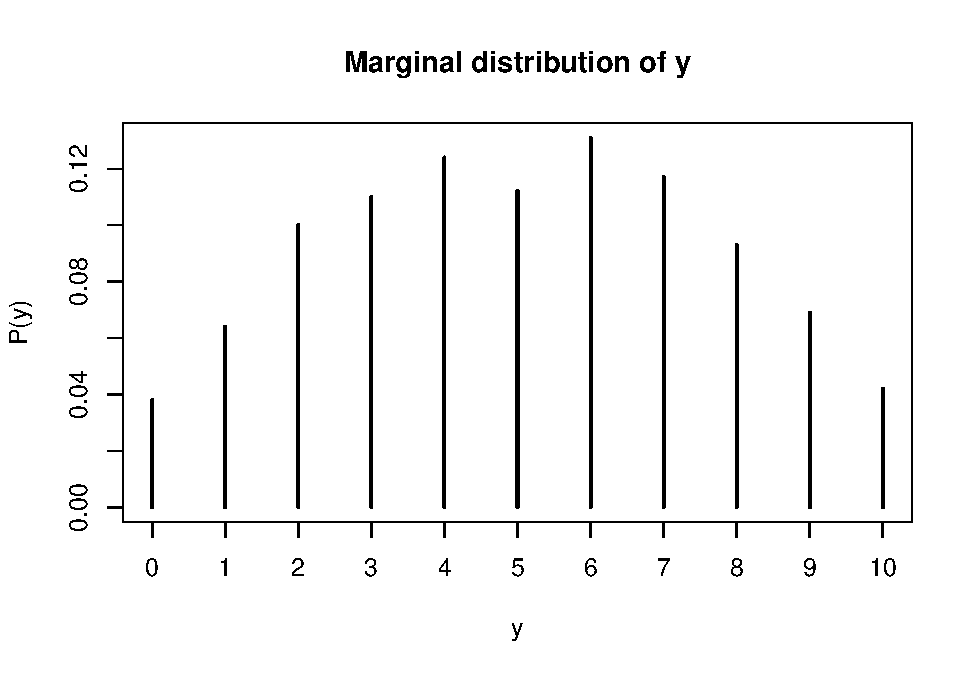
\includegraphics{bookdown-demo_files/figure-latex/unnamed-chunk-9-2.pdf}

\begin{Shaded}
\begin{Highlighting}[]
\CommentTok{# the marginal expected value of y}
\KeywordTok{mean}\NormalTok{(y)}
\end{Highlighting}
\end{Shaded}

\begin{verbatim}
## [1] 5.04
\end{verbatim}

\section{Markov chains}\label{markov-chains}

\subsection{Definition}\label{definition}

A sequence of random variable \(X_1, X_2,...,X_n\), with \(1, 2, ...,3\)
indicating the successitve points in time. Thus, based on the chain
rule, we can write the following:

\[p(X_1,X_2,...,X_n)=p(X_1)p(X_2|X_1)p(X_3|X_2,X_1)...p(X_n|X_{n-1},X_{n-2},...,X_2,X_1)\]

For Markov chains, it puts an assumption, called Markov assumption: The
random variable at the next time step only depends on the current
variable. Mathematically,

\[p(X_{t+1}|X_t,X_{t-1},...,X_2,X_1)=p(X_{t+1}|X_t)\]

where,

\[t=2, ...n\]

Thus, we can write the expression above as follows.

\[p(X_1,X_2,...,X_n)=p(X_1)p(X_2|X_1)p(X_3|X_2)P(X_4|X_3)...p(X_n|X_{n-1})\]

\subsection{Discrete example}\label{discrete-example}

Suppose that you flip a coin. You have a set of number \{1,2,3,4,5\}. If
it is head, you increase 1 in the next number (for instance, if you are
2 now, you will be get 3 in the next). In contrast, if it is tail, you
will decrease the number (e.g., 2 is now and 1 is next). If is is 5,
increase 1 will lead to 1. Logically, 1 and then it is reduced by 1,
leading to 5.

\subsection{Continuous example}\label{continuous-example}

\[p(X_{t+1}| X_t=x_t)=N(x_t,1)\]

\begin{Shaded}
\begin{Highlighting}[]
\KeywordTok{set.seed}\NormalTok{(}\DecValTok{123}\NormalTok{)}
\NormalTok{n=}\DecValTok{100}
\NormalTok{x=}\KeywordTok{numeric}\NormalTok{(n)}

\ControlFlowTok{for}\NormalTok{(i }\ControlFlowTok{in} \DecValTok{2}\OperatorTok{:}\NormalTok{n)}
\NormalTok{\{x[i]=}\KeywordTok{rnorm}\NormalTok{(}\DecValTok{1}\NormalTok{,}\DataTypeTok{mean=}\NormalTok{x[i}\OperatorTok{-}\DecValTok{1}\NormalTok{],}\DecValTok{1}\NormalTok{)\}}

\KeywordTok{plot.ts}\NormalTok{(x)}
\end{Highlighting}
\end{Shaded}

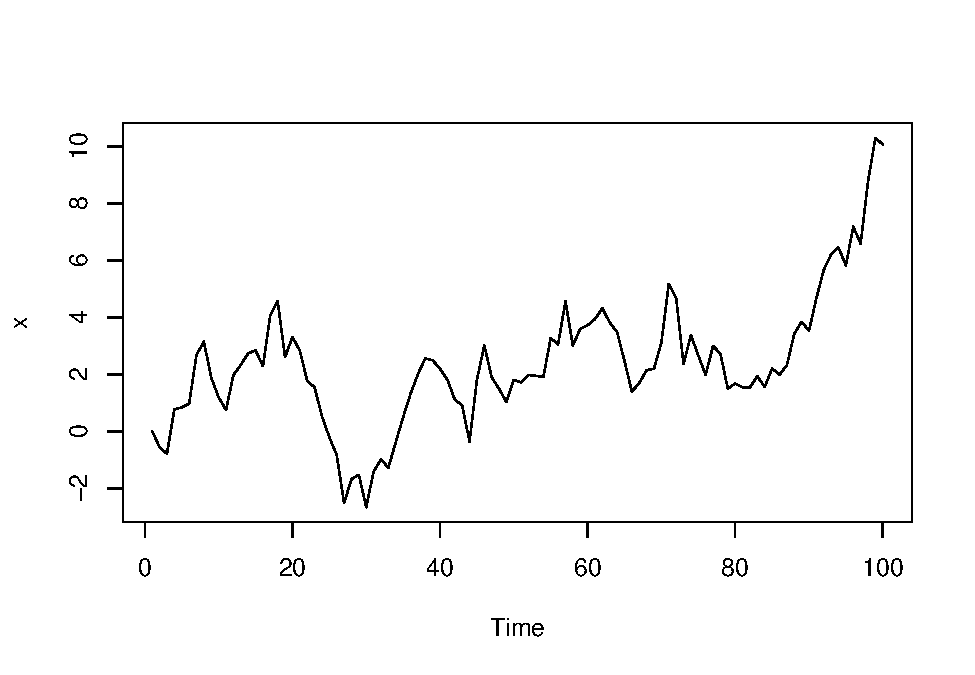
\includegraphics{bookdown-demo_files/figure-latex/unnamed-chunk-10-1.pdf}

\subsection{Discrete example and transition
matrix}\label{discrete-example-and-transition-matrix}

For the discrete example above, we can write the following transition
matrix. We know that \(p(X_{t+1}=5 | X_t=4)\) can be found in the 4th
row, 5th column, namely 0.5.

\[Q=\begin{bmatrix} 0 & 0.5 & 0 & 0 & 0.5 \\ 0.5 & 0 & 0.5 & 0 & 0\\ 0 & 0.5 & 0 & 0.5 & 0 \\ 0& 0 & 0.5& 0& 0.5\\ 0.5 & 0& 0 &0.5 & 0 \end{bmatrix}\]

The transition matrix is especially useful when there are mutiple steps
in the chain. such as \(p(X_{t+1}=5| X_t=4)\). It can be calculated as
\(\sum_{k=1}^{5} p(X_{t+2}=3|X_{t+1}=k) \cdot p(X_{t+1}=k |X_t=1)\). We
can use R code the impletement this.

\begin{Shaded}
\begin{Highlighting}[]
\NormalTok{Q =}\StringTok{ }\KeywordTok{matrix}\NormalTok{(}\KeywordTok{c}\NormalTok{(}\FloatTok{0.0}\NormalTok{, }\FloatTok{0.5}\NormalTok{, }\FloatTok{0.0}\NormalTok{, }\FloatTok{0.0}\NormalTok{, }\FloatTok{0.5}\NormalTok{,}
             \FloatTok{0.5}\NormalTok{, }\FloatTok{0.0}\NormalTok{, }\FloatTok{0.5}\NormalTok{, }\FloatTok{0.0}\NormalTok{, }\FloatTok{0.0}\NormalTok{,}
             \FloatTok{0.0}\NormalTok{, }\FloatTok{0.5}\NormalTok{, }\FloatTok{0.0}\NormalTok{, }\FloatTok{0.5}\NormalTok{, }\FloatTok{0.0}\NormalTok{,}
             \FloatTok{0.0}\NormalTok{, }\FloatTok{0.0}\NormalTok{, }\FloatTok{0.5}\NormalTok{, }\FloatTok{0.0}\NormalTok{, }\FloatTok{0.5}\NormalTok{,}
             \FloatTok{0.5}\NormalTok{, }\FloatTok{0.0}\NormalTok{, }\FloatTok{0.0}\NormalTok{, }\FloatTok{0.5}\NormalTok{, }\FloatTok{0.0}\NormalTok{), }
           \DataTypeTok{nrow=}\DecValTok{5}\NormalTok{, }\DataTypeTok{byrow=}\OtherTok{TRUE}\NormalTok{)}

\NormalTok{(jj<-Q }\OperatorTok\StringTok{ }\NormalTok{Q)}
\end{Highlighting}
\end{Shaded}

\begin{verbatim}
##      [,1] [,2] [,3] [,4] [,5]
## [1,] 0.50 0.00 0.25 0.25 0.00
## [2,] 0.00 0.50 0.00 0.25 0.25
## [3,] 0.25 0.00 0.50 0.00 0.25
## [4,] 0.25 0.25 0.00 0.50 0.00
## [5,] 0.00 0.25 0.25 0.00 0.50
\end{verbatim}

\begin{Shaded}
\begin{Highlighting}[]
\NormalTok{jj[}\DecValTok{1}\NormalTok{,}\DecValTok{3}\NormalTok{]}
\end{Highlighting}
\end{Shaded}

\begin{verbatim}
## [1] 0.25
\end{verbatim}

\subsection{Stationary distribution}\label{stationary-distribution}

\textbf{Discrete Cases}\_

\begin{Shaded}
\begin{Highlighting}[]
\NormalTok{Q5 =}\StringTok{ }\NormalTok{Q }\OperatorTok\StringTok{ }\NormalTok{Q }\OperatorTok\StringTok{ }\NormalTok{Q }\OperatorTok\StringTok{ }\NormalTok{Q }\OperatorTok\StringTok{ }\NormalTok{Q }\CommentTok{# h=5 steps in the future}

\NormalTok{Q5}
\end{Highlighting}
\end{Shaded}

\begin{verbatim}
##         [,1]    [,2]    [,3]    [,4]    [,5]
## [1,] 0.06250 0.31250 0.15625 0.15625 0.31250
## [2,] 0.31250 0.06250 0.31250 0.15625 0.15625
## [3,] 0.15625 0.31250 0.06250 0.31250 0.15625
## [4,] 0.15625 0.15625 0.31250 0.06250 0.31250
## [5,] 0.31250 0.15625 0.15625 0.31250 0.06250
\end{verbatim}

\begin{Shaded}
\begin{Highlighting}[]
\KeywordTok{round}\NormalTok{(Q5, }\DecValTok{3}\NormalTok{)}
\end{Highlighting}
\end{Shaded}

\begin{verbatim}
##       [,1]  [,2]  [,3]  [,4]  [,5]
## [1,] 0.062 0.312 0.156 0.156 0.312
## [2,] 0.312 0.062 0.312 0.156 0.156
## [3,] 0.156 0.312 0.062 0.312 0.156
## [4,] 0.156 0.156 0.312 0.062 0.312
## [5,] 0.312 0.156 0.156 0.312 0.062
\end{verbatim}

\begin{Shaded}
\begin{Highlighting}[]
\NormalTok{Q30 =}\StringTok{ }\NormalTok{Q}
\ControlFlowTok{for}\NormalTok{ (i }\ControlFlowTok{in} \DecValTok{2}\OperatorTok{:}\DecValTok{30}\NormalTok{) \{}
\NormalTok{  Q30 =}\StringTok{ }\NormalTok{Q30 }\OperatorTok\StringTok{ }\NormalTok{Q}
\NormalTok{\}}
\KeywordTok{round}\NormalTok{(Q30, }\DecValTok{3}\NormalTok{) }\CommentTok{# h=30 steps in the future}
\end{Highlighting}
\end{Shaded}

\begin{verbatim}
##       [,1]  [,2]  [,3]  [,4]  [,5]
## [1,] 0.201 0.199 0.200 0.200 0.199
## [2,] 0.199 0.201 0.199 0.200 0.200
## [3,] 0.200 0.199 0.201 0.199 0.200
## [4,] 0.200 0.200 0.199 0.201 0.199
## [5,] 0.199 0.200 0.200 0.199 0.201
\end{verbatim}

Thus, as we can see, as the time gap gets bigger, the transition
distributions appear to converge.

\begin{Shaded}
\begin{Highlighting}[]
\NormalTok{Q =}\StringTok{ }\KeywordTok{matrix}\NormalTok{(}\KeywordTok{c}\NormalTok{(}\FloatTok{0.0}\NormalTok{, }\FloatTok{0.5}\NormalTok{, }\FloatTok{0.0}\NormalTok{, }\FloatTok{0.0}\NormalTok{, }\FloatTok{0.5}\NormalTok{,}
             \FloatTok{0.5}\NormalTok{, }\FloatTok{0.0}\NormalTok{, }\FloatTok{0.5}\NormalTok{, }\FloatTok{0.0}\NormalTok{, }\FloatTok{0.0}\NormalTok{,}
             \FloatTok{0.0}\NormalTok{, }\FloatTok{0.5}\NormalTok{, }\FloatTok{0.0}\NormalTok{, }\FloatTok{0.5}\NormalTok{, }\FloatTok{0.0}\NormalTok{,}
             \FloatTok{0.0}\NormalTok{, }\FloatTok{0.0}\NormalTok{, }\FloatTok{0.5}\NormalTok{, }\FloatTok{0.0}\NormalTok{, }\FloatTok{0.5}\NormalTok{,}
             \FloatTok{0.5}\NormalTok{, }\FloatTok{0.0}\NormalTok{, }\FloatTok{0.0}\NormalTok{, }\FloatTok{0.5}\NormalTok{, }\FloatTok{0.0}\NormalTok{), }
           \DataTypeTok{nrow=}\DecValTok{5}\NormalTok{, }\DataTypeTok{byrow=}\OtherTok{TRUE}\NormalTok{)}
\NormalTok{Q}
\end{Highlighting}
\end{Shaded}

\begin{verbatim}
##      [,1] [,2] [,3] [,4] [,5]
## [1,]  0.0  0.5  0.0  0.0  0.5
## [2,]  0.5  0.0  0.5  0.0  0.0
## [3,]  0.0  0.5  0.0  0.5  0.0
## [4,]  0.0  0.0  0.5  0.0  0.5
## [5,]  0.5  0.0  0.0  0.5  0.0
\end{verbatim}

\begin{Shaded}
\begin{Highlighting}[]
\KeywordTok{c}\NormalTok{(}\FloatTok{0.2}\NormalTok{, }\FloatTok{0.2}\NormalTok{, }\FloatTok{0.2}\NormalTok{, }\FloatTok{0.2}\NormalTok{, }\FloatTok{0.2}\NormalTok{) }\OperatorTok\StringTok{ }\NormalTok{Q}
\end{Highlighting}
\end{Shaded}

\begin{verbatim}
##      [,1] [,2] [,3] [,4] [,5]
## [1,]  0.2  0.2  0.2  0.2  0.2
\end{verbatim}

The definition of stationary distribution of a chain:

The initial state distribution for which performing a transition will
not change the probability of ending up in any given state.

For a Markov chain after many iterations, the samples can be used as a
Monte Carlo sample from the stationary distribution. Thus, we can use
Markov chains for Bayesian inference. In order to simulate from a
complicated posterior distribution, we will set up and run a Markov
chain whose stationary distribution is the posterior distribution. (Note
that: stationary distribution doesn't always exist for any given Markov
chain)

\textbf{Continuous Cases}\_

As we can see, the example shown earlier does not reach a stationary
distribution. But, we can modify it to make it happen.

\[p(X_{t+1}|X_t=x_t)=N(\phi x_t,1), -1<\phi<1\]

It will reach a stationary distribution as long as \(-1<\phi<1\).

\begin{Shaded}
\begin{Highlighting}[]
\NormalTok{n =}\StringTok{ }\DecValTok{1000}
\NormalTok{x =}\StringTok{ }\KeywordTok{numeric}\NormalTok{(n)}
\NormalTok{phi =}\StringTok{ }\OperatorTok{-}\FloatTok{0.5}

\ControlFlowTok{for}\NormalTok{ (i }\ControlFlowTok{in} \DecValTok{2}\OperatorTok{:}\NormalTok{n) \{}
\NormalTok{  x[i] =}\StringTok{ }\KeywordTok{rnorm}\NormalTok{(}\DecValTok{1}\NormalTok{, }\DataTypeTok{mean=}\NormalTok{phi}\OperatorTok{*}\NormalTok{x[i}\OperatorTok{-}\DecValTok{1}\NormalTok{], }\DataTypeTok{sd=}\FloatTok{1.0}\NormalTok{)}
\NormalTok{\}}

\KeywordTok{plot.ts}\NormalTok{(x)}
\end{Highlighting}
\end{Shaded}

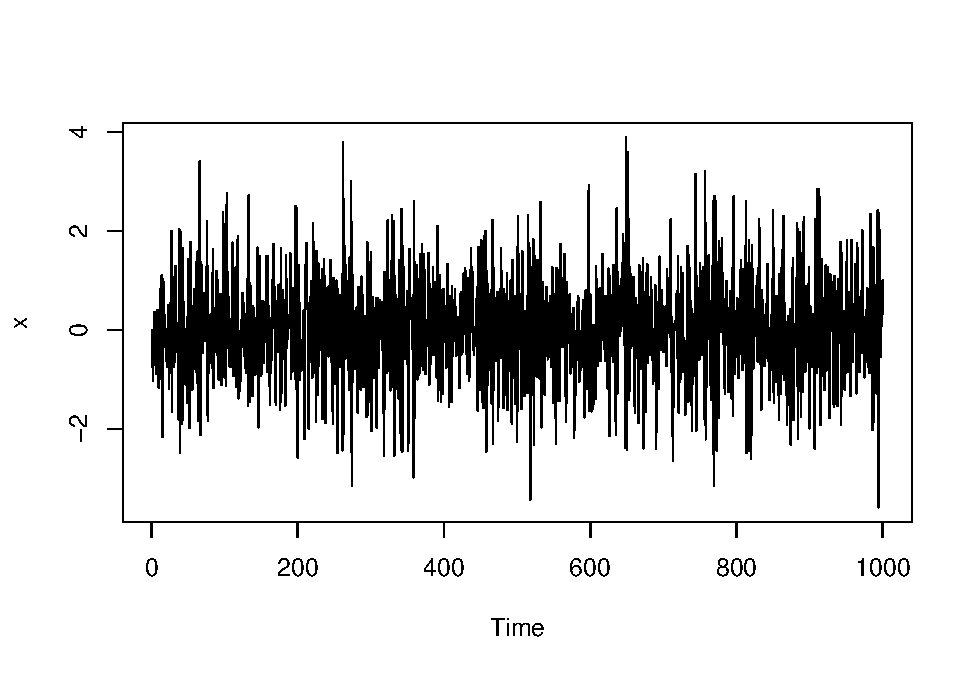
\includegraphics{bookdown-demo_files/figure-latex/unnamed-chunk-15-1.pdf}

\begin{Shaded}
\begin{Highlighting}[]
\KeywordTok{hist}\NormalTok{(x, }\DataTypeTok{freq=}\OtherTok{FALSE}\NormalTok{)}
\KeywordTok{curve}\NormalTok{(}\KeywordTok{dnorm}\NormalTok{(x, }\DataTypeTok{mean=}\FloatTok{0.0}\NormalTok{, }\DataTypeTok{sd=}\KeywordTok{sqrt}\NormalTok{(}\FloatTok{1.0}\OperatorTok{/}\NormalTok{(}\FloatTok{1.0}\OperatorTok{-}\NormalTok{phi}\OperatorTok{^}\DecValTok{2}\NormalTok{))), }\DataTypeTok{col=}\StringTok{"red"}\NormalTok{, }\DataTypeTok{add=}\OtherTok{TRUE}\NormalTok{)}
\KeywordTok{legend}\NormalTok{(}\StringTok{"topright"}\NormalTok{, }\DataTypeTok{legend=}\StringTok{"theoretical stationary}\CharTok{\textbackslash{}n}\StringTok{distribution"}\NormalTok{, }\DataTypeTok{col=}\StringTok{"red"}\NormalTok{, }\DataTypeTok{lty=}\DecValTok{1}\NormalTok{, }\DataTypeTok{bty=}\StringTok{"n"}\NormalTok{)}
\end{Highlighting}
\end{Shaded}

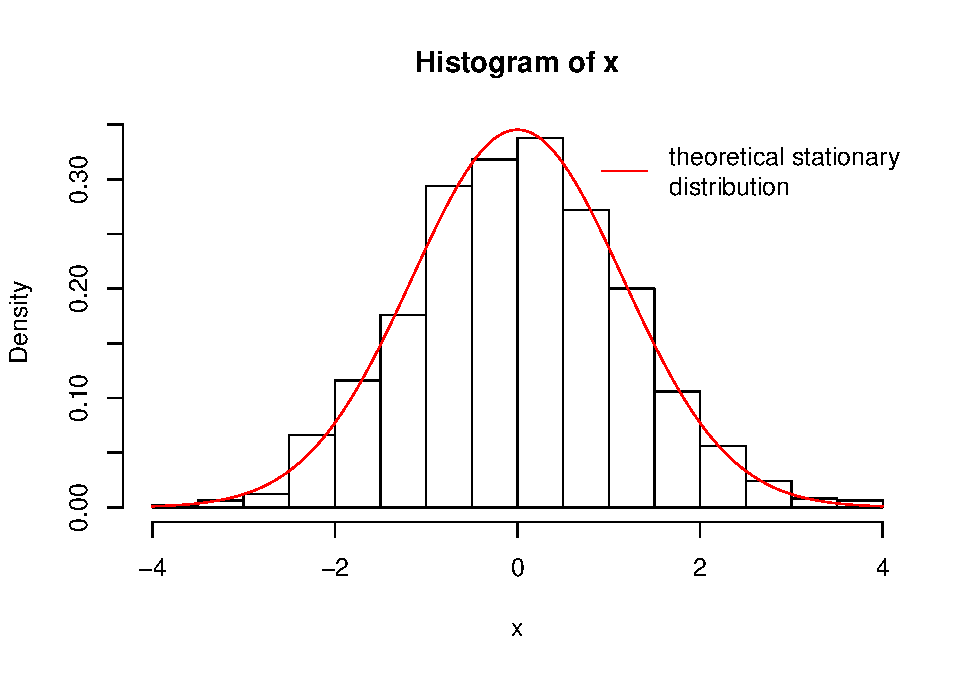
\includegraphics{bookdown-demo_files/figure-latex/unnamed-chunk-15-2.pdf}

It will reach the stationary distribution of
\(N(0, \frac{1}{1-\phi^2})\)

\section{Metropolis-Hastings}\label{metropolis-hastings}

\subsection{Procedure}\label{procedure}

\begin{enumerate}
\def\labelenumi{(\arabic{enumi})}
\item
  Select initial value \(\theta_0\)
\item
  For \(i=1,..., m\), repeat:
\end{enumerate}

\begin{enumerate}
\def\labelenumi{(\alph{enumi})}
\item
  Draw candidate \(\theta^* \sim q(\theta^*|\theta_{i-1})\)
\item
  \(\alpha=\frac{g(\theta^*)/q(\theta^*|\theta_{i-1})}{g(\theta_{i-1})/q(\theta_{i-1}|\theta^*)}=\frac{g(\theta^*)q(\theta_{i-1}|\theta^*)}{g(\theta_{i-1})q(\theta^*|\theta_{i-1})}\)
\item
  \(\alpha \geq 1\) accept \(\theta^*\) and set
  \(\theta_i \leftarrow \theta^*\)
\end{enumerate}

\(0<\alpha < 1\) accept \(\theta^*\) and set
\(\theta_i \leftarrow \theta^*\) with probablity \(\alpha\)

\subsection{Demonstration}\label{demonstration}

Prior \(P(loaded)=0.6\)

\[\begin{aligned} f(\theta | X) &= \frac{f(x|\theta) f(\theta)}{\sum_{\theta} f(x|\theta)f(\theta)} \\ &=\frac{\binom{5}{x} [(\frac{1}{2})^5 \times 0.4 \times I_{\{\theta=fair \}}+ (0.7)^x(0.3)^{5-x} \times 0.6 \times I_{\{\theta=loaded \}}]}{\binom{5}{x} [(\frac{1}{2})^5 \times 0.4 + (0.7)^x(0.3)^{5-x} \times 0.6]}  \end{aligned}\]

\[\begin{aligned} f(\theta |X=2) &=\frac{0.0125 I_{\{\theta=fair \}}+0.0079 I_{\{\theta=loaded \}} }{0.0125+0.0079} \\ &= 0.612 I_{\{\theta=fair \}} + 0.388 I_{\{\theta=loaded \}} \end{aligned}\]
Thus, we can say that:

\[P(\theta=loaded | X=2)=0.388\]

\begin{enumerate}
\def\labelenumi{(\arabic{enumi})}
\item
  Start at either \(\theta_0=fair\) or \(\theta_0=loaded\)
\item
  For \(i=1, ...m\)
\end{enumerate}

\begin{enumerate}
\def\labelenumi{(\alph{enumi})}
\item
  Propose candidate \(\theta^*\) to be the other state such as
  \(\theta_{i-1}\)
\item
\end{enumerate}

\[\alpha=\frac{g(\theta^*)/q(\theta^*|\theta_{i-1})}{g(\theta_{i-1})/q(\theta_{i-1}|\theta^*)}=\frac{f(x=2|\theta^*)/1}{f(x=2|\theta_{i-1})/1}\]

If \(\theta^*=loaded, \alpha=\frac{0.0794}{0.0125}=0.635\) If
\(\theta^*=fair, \alpha=\frac{0.0125}{0.0794}=1.574\)

\begin{enumerate}
\def\labelenumi{(\alph{enumi})}
\setcounter{enumi}{2}
\tightlist
\item
  if \(\theta^*=fair, \alpha>1\), accept \(\theta^*\) set
  \(\theta_i=fair\)
\end{enumerate}

if \(\theta^*=loaded, \alpha>0.635\), accept \(\theta^*\) set
\(\theta_i=loaded\) w.p.~0.635.

Thus, we can get the following transition matrix:

\[Q=\begin{bmatrix} 0.365 & 0.635  \\ 1 & 0  \end{bmatrix}\]

This means that:

\begin{enumerate}
\def\labelenumi{(\arabic{enumi})}
\item
  When \(\theta_{i-1}\) is fair, \(\theta_{i}\) is also fair, the
  \(P=0.365\).
\item
  When \(\theta_{i-1}\) is fair, \(\theta_{i}\) is loaded, the
  \(P=0.635\).
\item
  When \(\theta_{i-1}\) is loaded, \(\theta_{i}\) is fair, the \(P=1\).
\item
  When \(\theta_{i-1}\) is loaded, \(\theta_{i}\) is loaded, the
  \(P=0\).
\end{enumerate}

Thus,

\[\pi = [0.612, 0.388]\]

\[[0.612, 0.388]\begin{bmatrix} 0.365 & 0.635  \\ 1 & 0  \end{bmatrix}=[0.612, 0.388]\]

\subsection{R code}\label{r-code}

The data are the percent change in total personnel for n=10 companies
(1.2,1.4,-0.5,0.3,0.9,2.3,1.0,0.1,1.3,1.9). We assume such changes
follow a normal distribution with known variance (but mean is unknown).
For the mean (i.e., \(\mu\)), we assume it follows a t distribution
(i.e., the prior for the \(\mu\) is t-distribution).Since t-distribution
prior is not conjugate to a normal distribution, the posterior
distribution is not in a standard form that we can easily sample. Thus,
we need to set up a Markov chain whose stationary distribution is the
posterior distribution.

\[p(\mu|y_1,...,y_n) \propto \frac{exp[n(\bar{y}\mu-\mu^2/2)]}{1+\mu^2}\]

\[log(g(\mu))=n(\bar{y}\mu-\mu^2/2)-log(1+\mu^2)\]

\begin{Shaded}
\begin{Highlighting}[]
\NormalTok{lg=}\ControlFlowTok{function}\NormalTok{(mu, n, ybar)}
\NormalTok{\{ mu2=mu}\OperatorTok{^}\DecValTok{2}
\NormalTok{  n}\OperatorTok{*}\NormalTok{(ybar}\OperatorTok{*}\NormalTok{mu}\OperatorTok{-}\NormalTok{mu2}\OperatorTok{/}\DecValTok{2}\NormalTok{)}\OperatorTok{-}\KeywordTok{log}\NormalTok{(}\DecValTok{1}\OperatorTok{+}\NormalTok{mu2)\}}

\NormalTok{mu_now=}\DecValTok{10}
\NormalTok{cand_sd=}\DecValTok{5}
\NormalTok{y=}\KeywordTok{c}\NormalTok{(}\FloatTok{1.2}\NormalTok{,}\FloatTok{1.4}\NormalTok{,}\OperatorTok{-}\FloatTok{0.5}\NormalTok{,}\FloatTok{0.3}\NormalTok{,}\FloatTok{0.9}\NormalTok{,}\FloatTok{2.3}\NormalTok{,}\FloatTok{1.0}\NormalTok{,}\FloatTok{0.1}\NormalTok{,}\FloatTok{1.3}\NormalTok{,}\FloatTok{1.9}\NormalTok{)}
\NormalTok{ybar=}\KeywordTok{mean}\NormalTok{(y)}

\NormalTok{mh<-}\ControlFlowTok{function}\NormalTok{(mu_now,type_MH,cand_sd)}
\NormalTok{\{}
\NormalTok{m=}\DecValTok{1000}
\NormalTok{n=}\KeywordTok{length}\NormalTok{(y)}
\NormalTok{mu_storage<-}\KeywordTok{c}\NormalTok{()}
\NormalTok{mu_storage<-}\KeywordTok{c}\NormalTok{(mu_storage,mu_now)}
\NormalTok{acceptance_count=}\DecValTok{0}

\ControlFlowTok{for}\NormalTok{ (i }\ControlFlowTok{in} \DecValTok{1}\OperatorTok{:}\NormalTok{m)}
\NormalTok{\{}
  \ControlFlowTok{if}\NormalTok{ (type_MH}\OperatorTok{==}\StringTok{"randomwalk"}\NormalTok{)  }\CommentTok{# random walk}
\NormalTok{  \{}
\NormalTok{  mu_cand =}\StringTok{ }\KeywordTok{rnorm}\NormalTok{(}\DataTypeTok{n=}\DecValTok{1}\NormalTok{, }\DataTypeTok{mean=}\NormalTok{mu_now, }\DataTypeTok{sd=}\NormalTok{cand_sd)}
\NormalTok{  \}}
  \ControlFlowTok{else}
\NormalTok{  \{}
    \ControlFlowTok{if}\NormalTok{(type_MH}\OperatorTok{==}\StringTok{"independent"}\NormalTok{)  }\CommentTok{# independent, as mean is fixed}
\NormalTok{    \{mu_cand =}\StringTok{ }\KeywordTok{rnorm}\NormalTok{(}\DataTypeTok{n=}\DecValTok{1}\NormalTok{, }\DataTypeTok{mean=}\DecValTok{3}\NormalTok{, }\DataTypeTok{sd=}\NormalTok{cand_sd)\}}
    \ControlFlowTok{else}
\NormalTok{    \{}\KeywordTok{print}\NormalTok{(}\StringTok{"woring type of MH"}\NormalTok{)}
     \ControlFlowTok{break}
\NormalTok{    \}}
\NormalTok{  \}}
  
\NormalTok{  lg_alpha=}\KeywordTok{lg}\NormalTok{(mu_cand,}\DataTypeTok{n=}\NormalTok{n,}\DataTypeTok{ybar =}\NormalTok{ ybar)}\OperatorTok{-}\KeywordTok{lg}\NormalTok{(mu_now,}\DataTypeTok{n=}\NormalTok{n,}\DataTypeTok{ybar=}\NormalTok{ybar)}
\NormalTok{  alpha=}\KeywordTok{exp}\NormalTok{(lg_alpha)}
  \ControlFlowTok{if}\NormalTok{(alpha}\OperatorTok{>}\DecValTok{1}\NormalTok{)}
\NormalTok{    \{mu_now=mu_cand}
\NormalTok{    mu_storage<-}\KeywordTok{c}\NormalTok{(mu_storage,mu_cand)}
\NormalTok{    acceptance_count=acceptance_count}\OperatorTok{+}\DecValTok{1}\NormalTok{\}}
  \ControlFlowTok{else}
\NormalTok{    \{random_p=}\KeywordTok{runif}\NormalTok{(}\DecValTok{1}\NormalTok{)}
    \ControlFlowTok{if}\NormalTok{(alpha}\OperatorTok{>}\NormalTok{random_p)}
\NormalTok{      \{mu_now=mu_cand}
\NormalTok{      acceptance_count=acceptance_count}\OperatorTok{+}\DecValTok{1}\NormalTok{\}}
    \ControlFlowTok{else}
\NormalTok{      \{mu_now=mu_now\}}
\NormalTok{    \}}
\NormalTok{\}}

\KeywordTok{list}\NormalTok{(}\DataTypeTok{mu=}\NormalTok{mu_storage,}\DataTypeTok{accpt=}\NormalTok{acceptance_count}\OperatorTok{/}\NormalTok{m)}
\NormalTok{\}}

\NormalTok{tt_}\DecValTok{0}\NormalTok{<-}\KeywordTok{mh}\NormalTok{(}\DataTypeTok{mu_now=}\DecValTok{5}\NormalTok{,}\DataTypeTok{type_MH=}\StringTok{"randomwalk"}\NormalTok{,}\DataTypeTok{cand_sd=}\DecValTok{10}\NormalTok{)}
\KeywordTok{plot.ts}\NormalTok{(tt_}\DecValTok{0}\OperatorTok{$}\NormalTok{mu)}
\end{Highlighting}
\end{Shaded}

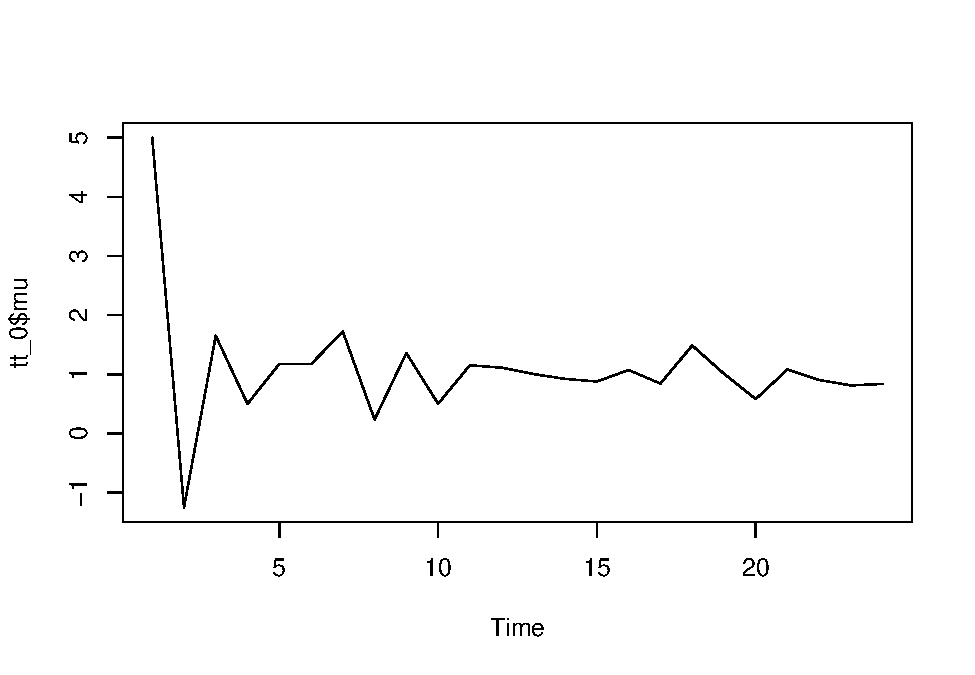
\includegraphics{bookdown-demo_files/figure-latex/unnamed-chunk-16-1.pdf}

\begin{Shaded}
\begin{Highlighting}[]
\NormalTok{tt_}\DecValTok{0}\OperatorTok{$}\NormalTok{accpt}
\end{Highlighting}
\end{Shaded}

\begin{verbatim}
## [1] 0.039
\end{verbatim}

\begin{Shaded}
\begin{Highlighting}[]
\NormalTok{tt_}\DecValTok{1}\NormalTok{<-}\KeywordTok{mh}\NormalTok{(}\DataTypeTok{mu_now=}\DecValTok{5}\NormalTok{,}\DataTypeTok{type_MH=}\StringTok{"randomwalk"}\NormalTok{,}\DataTypeTok{cand_sd=}\FloatTok{0.005}\NormalTok{)}
\KeywordTok{plot.ts}\NormalTok{(tt_}\DecValTok{1}\OperatorTok{$}\NormalTok{mu)}
\end{Highlighting}
\end{Shaded}

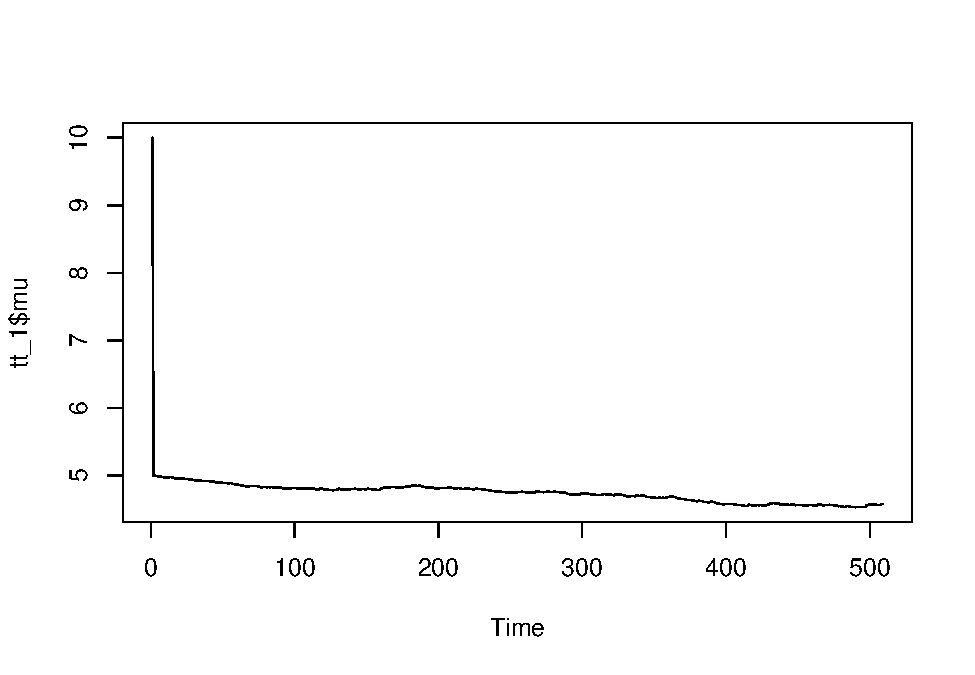
\includegraphics{bookdown-demo_files/figure-latex/unnamed-chunk-16-2.pdf}

\begin{Shaded}
\begin{Highlighting}[]
\NormalTok{tt_}\DecValTok{1}\OperatorTok{$}\NormalTok{accpt}
\end{Highlighting}
\end{Shaded}

\begin{verbatim}
## [1] 0.931
\end{verbatim}

\begin{Shaded}
\begin{Highlighting}[]
\NormalTok{tt_}\DecValTok{2}\NormalTok{<-}\KeywordTok{mh}\NormalTok{(}\DataTypeTok{mu_now=}\DecValTok{5}\NormalTok{,}\DataTypeTok{type_MH=}\StringTok{"randomwalk"}\NormalTok{,}\DataTypeTok{cand_sd=}\FloatTok{0.5}\NormalTok{)}
\KeywordTok{plot.ts}\NormalTok{(tt_}\DecValTok{2}\OperatorTok{$}\NormalTok{mu)}
\end{Highlighting}
\end{Shaded}

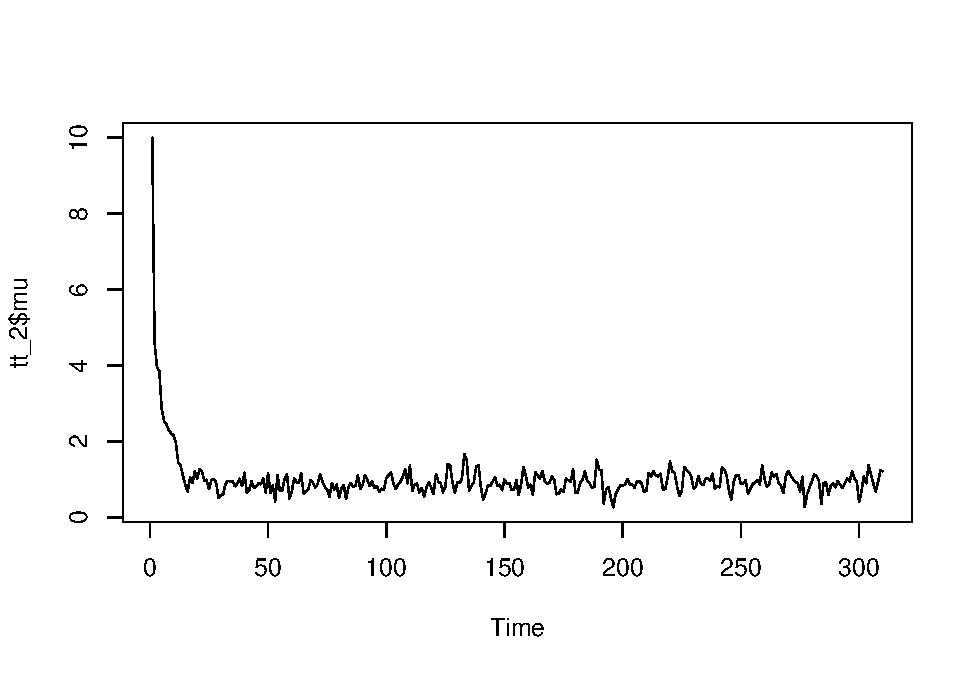
\includegraphics{bookdown-demo_files/figure-latex/unnamed-chunk-16-3.pdf}

\begin{Shaded}
\begin{Highlighting}[]
\NormalTok{tt_}\DecValTok{2}\OperatorTok{$}\NormalTok{accpt}
\end{Highlighting}
\end{Shaded}

\begin{verbatim}
## [1] 0.587
\end{verbatim}

As we can see, when the variance is big, the acceptance rate is low.
When the variance is low, in conrast, the acceptance rate is high. Note
that, changing the mean does not change the acceptance rate too much. In
the following, I plotted the prior, posteior, and the sample(i.e.,
\(y\)).

\begin{Shaded}
\begin{Highlighting}[]
\NormalTok{mu_keep<-tt_}\DecValTok{2}\OperatorTok{$}\NormalTok{mu[}\OperatorTok{-}\KeywordTok{c}\NormalTok{(}\DecValTok{1}\OperatorTok{:}\DecValTok{2}\NormalTok{)]}
\KeywordTok{plot}\NormalTok{(}\KeywordTok{density}\NormalTok{(mu_keep),}\DataTypeTok{xlim=}\KeywordTok{c}\NormalTok{(}\OperatorTok{-}\DecValTok{3}\NormalTok{,}\DecValTok{6}\NormalTok{))}
\KeywordTok{curve}\NormalTok{(}\KeywordTok{dt}\NormalTok{(x,}\DataTypeTok{df=}\DecValTok{1}\NormalTok{),}\DataTypeTok{lty=}\DecValTok{2}\NormalTok{,}\DataTypeTok{add =} \OtherTok{TRUE}\NormalTok{,}\DataTypeTok{col=}\StringTok{"red"}\NormalTok{)}
\KeywordTok{legend}\NormalTok{(}\StringTok{"topright"}\NormalTok{,}\DataTypeTok{legend=}\KeywordTok{c}\NormalTok{(}\StringTok{"Prior t-distribution pdf"}\NormalTok{, }\StringTok{"Posterior pdf"}\NormalTok{), }\DataTypeTok{col=}\KeywordTok{c}\NormalTok{(}\StringTok{"red"}\NormalTok{,}\StringTok{"black"}\NormalTok{), }\DataTypeTok{lty=}\DecValTok{1}\NormalTok{, }\DataTypeTok{bty=}\StringTok{"n"}\NormalTok{)}
\KeywordTok{points}\NormalTok{(ybar,}\DecValTok{0}\NormalTok{,}\DataTypeTok{pch=}\DecValTok{20}\NormalTok{)}
\KeywordTok{legend}\NormalTok{(}\DecValTok{1}\NormalTok{,}\DecValTok{1}\NormalTok{, }\DataTypeTok{legend=}\StringTok{"The black dot is the mean of y"}\NormalTok{,}\DataTypeTok{bty=}\StringTok{"n"}\NormalTok{)}
\end{Highlighting}
\end{Shaded}

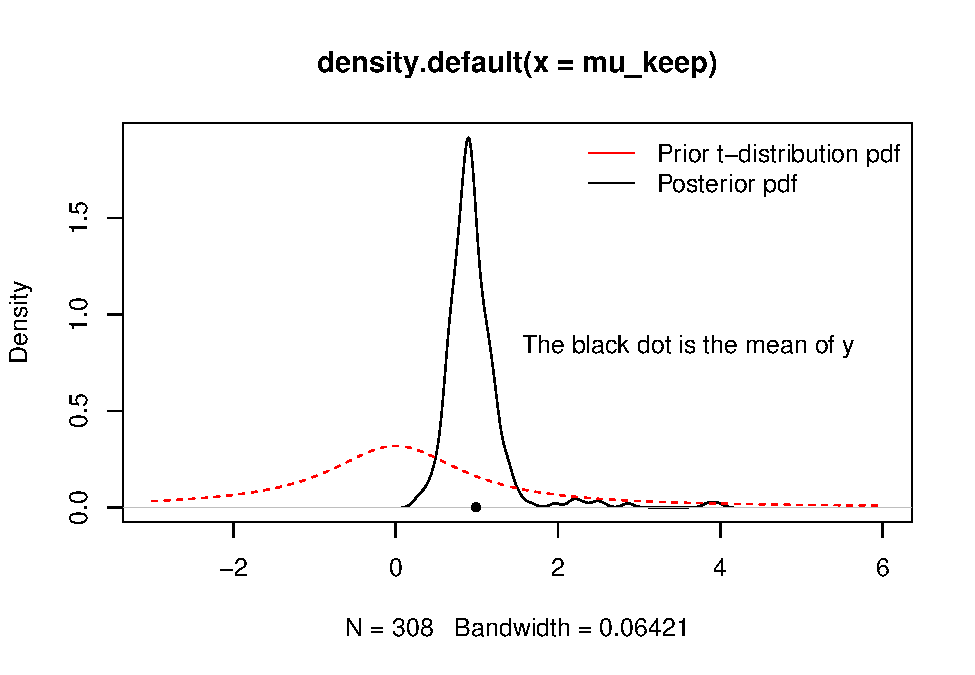
\includegraphics{bookdown-demo_files/figure-latex/unnamed-chunk-17-1.pdf}

In the following, I show the situation that the proposal distribution is
not random walk, but rather independent. That is, the mean for the
normal distribution is fixed. Refer to the procedure of MH, there is a
setence of:

\textbf{Draw candidate \(\theta^* \sim q(\theta^*|\theta_{i-1})\)}

\begin{Shaded}
\begin{Highlighting}[]
\NormalTok{tt_}\DecValTok{3}\NormalTok{<-}\KeywordTok{mh}\NormalTok{(}\DataTypeTok{mu_now=}\DecValTok{5}\NormalTok{,}\DataTypeTok{type_MH=}\StringTok{"independent"}\NormalTok{,}\DataTypeTok{cand_sd=}\FloatTok{0.5}\NormalTok{)}
\KeywordTok{plot.ts}\NormalTok{(tt_}\DecValTok{3}\OperatorTok{$}\NormalTok{mu)}
\end{Highlighting}
\end{Shaded}

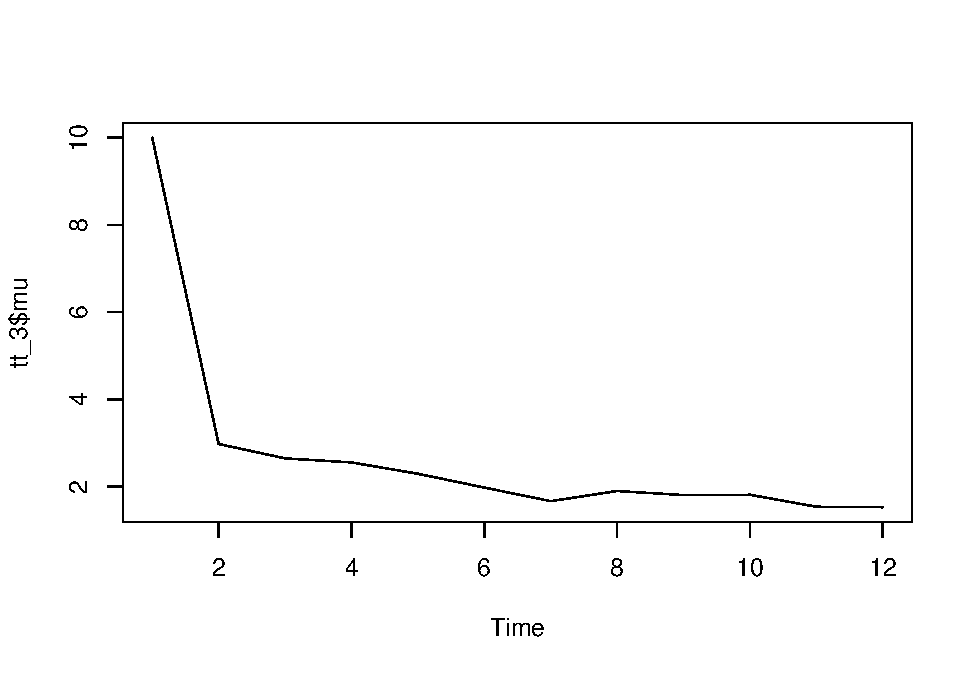
\includegraphics{bookdown-demo_files/figure-latex/unnamed-chunk-18-1.pdf}

\begin{Shaded}
\begin{Highlighting}[]
\NormalTok{tt_}\DecValTok{3}\OperatorTok{$}\NormalTok{accpt}
\end{Highlighting}
\end{Shaded}

\begin{verbatim}
## [1] 0.016
\end{verbatim}

\begin{Shaded}
\begin{Highlighting}[]
\CommentTok{#tt_4<-mh(mu_now=5,type_MH="hello",cand_sd=0.5)}
\CommentTok{#tt_4}
\end{Highlighting}
\end{Shaded}

\bibliography{book.bib,packages.bib}

\end{document}
